\chapter{Measurement of the inclusive \ttbartitle cross section at \texorpdfstring{\sqrtsRIII}{sqrt(s) = 13 TeV}}
\label{ch:ttxs}

This chapter describes the measurement of the inclusive \ttbar production cross section at the LHC at the center-of-mass energy of \sqrtsRIII. First, a motivation and overview of the analysis design will be given. Then, object and cut definitions as well as several applied corrections will be explained in detail. Finally, the likelihood fit used to extract the cross section, including all uncertainties, is described and the result discussed.

\section{Introduction}

% motivation: new com energy, possible glimpse at new physics; new run, new calibrations, top physics requires most objects -> good check of performance

% method needs to be tuned for early measurement
% special mention: lepton sf -> can be estimated in situ
% do one fit with and one without

In July 2022, the LHC officially resumed collecting data after a roughly three-year technical stop, thereby starting LHC Run 3. It did so at a new, unprecedented center-of-mass energy of \sqrtsRIII, inviting the experiments to measure energy-dependent physical observables at the new energy frontier.

One important such observable is the inclusive \ttbar production cross section. As mentioned in Ch. \ref{ch:theory}, the top quark has a special place in the standard model as the heaviest known elementary particle, as well as the only colored particle that does not hadronize due to its short lifetime. It is thus important for many BSM scenarios such as additional Higgs bosons, which might couple strongly to the top quark. As such, measurements of top-related observables at the highest possible energies can be used to test the Standard Model. The inclusive \ttbar cross section, as one of the simplest top quark observables, is well suited for a first measurement at the new center-of-mass energy.

Simultaneously, restarting such a large experiment as the CMS detector after a three-year technical stop poses many experimental challenges. Due to the change in energy, as well as physical changes in the accelerator and detector, most calibrations and corrections used to correctly describe the recorded data in simulation need to be re-derived and validated. An early measurement of the inclusive \ttbar cross section is well suited to cross-check this: Because of the decay chain of the top quark, a top-related measurement involves several of the different objects reconstructed at CMS, 
%, as described in Ch. \ref{sec:methods:reco}, 
enabling a check of a wide landscape of calibrations.

The measurement described in this chapter was designed specifically with these motivations in mind, and as such exhibits several novel features. Firstly, it combines events from both the dilepton and \ljets decay channels of \ttbar, categorized by lepton flavor content, combining the higher statistics of the \ljets channel with the high purity of the \emu channel and allowing to constrain uncertainties on the lepton identification efficiency directly from the data. This is done using a simultaneous maximum likelihood fit to the event yields in the different categories, with experimental and theoretical uncertainties treated as nuisance parameters.

Secondly, the events are additionally categorized by their number of b-tagged jets, which similarly allows for an in-situ measurement of the b-tagging efficiencies. This prevents the need to wait for external b-tagging calibrations, making for the earliest possible measurement.

The results of this work were first presented as a Physics Analysis Summary in September~2022~\cite{CMS:TOP-22-012-PAS}, only two months after the start of datataking, as the first public physics result of LHC Run~3. It was later published in \textit{JHEP} as \citere{CMS:TOP-22-012}, again representing the first published Run~3 result. A similar result by ATLAS was later published in \citere{ATLAS:2023slx}.

\section{Datasets and event selection}

In this section, the choice of datasets for experimental data and for simulation, as well as the choice of triggers, is described. Following that, the object and event selection procedure is outlined and several event categories, to be used in the likelihood fit (\cref{sec:ttxs:fitresults}), are defined. 

\subsection{Datasets}
\label{sec:ttxs:datasets}

\paragraph{Experimental data}
The measurement is performed on data recorded during the period between July 27\textsuperscript{th} and August 02\textsuperscript{nd} 2022 (part of Era C of year 2022), corresponding to an integrated luminosity of \lumiRIII. This amount of data is chosen as a balance between sensitivity and speed for the early measurement: It roughly corresponds to the point where data statistics no longer significantly limit the measurement uncertainty, while at the same time it is not required to study calibrations at different beam and detector conditions (e.g. average pileup, which changed during the different eras of 2022).

% TODO luminosity measurement

Both single-lepton and dilepton triggers were used to select events used in this measurement during detector operation, identifying leptons in the range of $\abseta < 2.5$. The \pt requirements of the triggers are summarized in Tab.~\ref{tab:ttxs:triggers}.

\begin{table}
    \centering
    \begin{tabular}{c|c}
        Trigger & Lepton requirement \\
        \hline
        single-e & e($\pt > 32$ GeV) \\
        single-$\mu$ & $\mu$($\pt > 27$ GeV) \\
        ee & e($\pt > 23$ GeV) and e($\pt > 12$ GeV) \\
        $\mu\mu$ & $\mu$($\pt > 17$ GeV) and $\mu$($\pt > 8$ GeV) \\
        e$\mu$ & e($\pt > 23$ GeV) and $\mu$($\pt > 8$ GeV)  or \\
        & e($\pt > 12$ GeV) and $\mu$($\pt > 23$ GeV) \\
    \end{tabular}
    \caption{Trigger definitions used for the \ttbar cross section measurement. The leptons are required to be isolated and in the pseudorapidity range  $\abseta < 2.5$.}
    \label{tab:ttxs:triggers}
\end{table}

\paragraph{Simulation}
To compare the data with predictions, Monte Carlo (MC) simulation is used to simulate both the \ttbar signal as well as most important background processes, specifically single-top quark production in the $t$-channel, associated tW-production, Z+jets production, W+jets production, and diboson (WW, WZ and ZZ) production. The MC generator \textsc{Powheg v2}~\cite{Powheg:2004, Powheg:2007, Powheg:2010} is used to generate \ttbar, single-top, and tW events at next-to-leading order (NLO) in perturbative QCD, while the generators \textsc{MadGraph5\_aMC@NLO}~\cite{MG5aMCatNLO:2014} and \textsc{Pythia 8}~\cite{Pythia:2015} are used to generate Z+jets/W+jets and diboson events, respectively, at leading order (LO). For $t$-channel single-top, specifically, \textsc{MadSpin} is used to simulate the top decay.

All of the generated events are interfaced to \textsc{Pythia 8} for parton showering and hadronization, using the MLM prescription in the case of the samples produced with \textsc{MadGraph}, and further processed in a full simulation of the CMS detector using \textsc{Geant 4}~\cite{GEANT4:2002}. The proton structure in the matrix element calculation is described by the NNPDF3.1 parton distribution function (PDF) set at NNLO. Note that another background contribution, from QCD events with fake or non-prompt leptons, is not simulated, but estimated from data (see \cref{sec:ttxs:datadriven}).

Theoretical predictions, as well as the measured integrated luminosity, are used to normalize the cross sections of the signal and background samples as follows: The \ttbar signal, computed at NNLO+NLLL in QCD, is normalized to a cross section of \xsecpred, which is also used as prediction for comparison with the SM. For the other backgrounds, the following orders in QCD and methods or programs are used: \textsc{MCFM}~\cite{Campbell:2020fhf} (NNLO) for single-top, \textsc{DYTurbo}~\cite{Camarda:2019zyx} (NNLO) for W+jets and Z+jets, \textsc{Matrix}~\cite{Grazzini:2017mhc} (NLO) for diboson, and an NNLO calculation from Ref. \cite{Kidonakis:2021vob} for tW.


\subsection{Object definition}
\label{sec:ttxs:objects}

\paragraph{Leptons}

Electrons or muons are considered for the analysis if they have $\pt > 10$ GeV and $\abseta < 2.4$. For electrons, the range $1.44 < \abseta < 1.57$, corresponding to the transition region between barrel and endcaps in the ECAL, is removed. Furthermore, additional identification criteria (ID) are applied to remove non-prompt or fake (i.e. wrongly reconstructed) leptons and enrich the selection with \ttbar events.

For electrons, the "tight" working point of the cut-based ID described in \citere{CMS:EGM-17-001} is applied, which includes information from both the details of the electromagnetic shower in the ECAL and the track, as well as the matching between the two. It also includes a requirement for the electron to be isolated from other particles such as hadrons, which is implemented in the form of the relative isolation variable. It is defined as the scalar \pt sum of all particles in a cone around the lepton in question, divided by the lepton \pt. Here, $\Delta R = \sqrt{(\Delta \eta)^2 + (\Delta \phi)^2} < 0.3$ is used for the radius of the cone. Additional corrections accounting for pileup particles are applied.

For muons, a similar cut-based ID is used as described in \citere{CMS:MUO-16-001}, also at the tight working point. Here, criteria on the compability of tracks in the innter tracker, the muon detectors and the reconstructed primary vertex are employed. Again, a cut on the relative isolation variable is used, defined equivalently but with a cone size of $\Delta R < 0.4$.

\paragraph{Jets}

The anti-$k_T$ algorithm~\cite{Cacciari:2008gp} is used to cluster reconstructed particles into jets with a distance parameter of 0.4. In order for a jet to be considered, it is required to have $\pt > 30$ GeV and $\abseta < 2.4$, and jets overlapping with any considered leptons (i.e. fulfilling the above criteria) are removed. %Again, additional ID criteria, based on the fractions of \pt originating from neutral hadron, charged hadron and electromagnetic jet constituents, are used to reject 

\paragraph{Tagging of b jets}

A special role is played by jets originating from the showering and hadronization of b quarks. Naively, two such jets are expected per \ttbar event from the two top decays, although in practice one or both jets may fall out of acceptance of the detector or otherwise not get identified, and conversely additional b quarks may be produced by radiation at higher orders in QCD. Correctly tagging these jets as such can greatly improve signal purity by cutting away backgrounds such as Z+jets, W+jets and QCD multijet events.

Here, the \textsc{DeepJet} algorithm is used to tag b jets, which is based on a deep neural network (DNN) classifier~\cite{DeepJet:2020,CMS:BTV-16-002}. A working point with an identification efficiency of more then 75 \% is used, with misidentification rates of around 17 \% for c jets and around 1 \% for other jets (i.e. from light quarks or gluons).

\subsection{Channel definition}
\label{sec:ttxs:channels}

Events are selected with either one or two leptons, corresponding respectively to the dilepton and \ljets decay channels of \ttbar. They are categorized into lepton channels by their lepton flavor content, and additional requirements are applied for the different channels. 

\paragraph{Dilepton channels}

Events with exactly two leptons, required to have opposite electric charge, are sorted into three dilepton channels (\emu, \ee, and \mumu). The presence of at least one jet is required, and in the same-flavor channels (\ee and \mumu), at least one jet is required to be b tagged in order to reject Z+jets and QCD multijet background. In the much purer \emu channel, on the other hand, events without b tags are retained to later help constrain the b tagging efficiency in the fit to data.

In order to reject even more Z+jets background, events in the same-flavor channels with an invariant dilepton mass of $| \mll - m_Z | < 15$ GeV, where $m_Z$ is the Z boson mass, are removed.

\paragraph{\ljets channels}

Events with exactly one lepton are sorted into the \ejets or \mujets channels based on their flavor. At least three jets are required, of which at least one needs to be b tagged. Note that regardless of these selections, there is still non-negligible background from QCD multijet events where the lepton is non-prompt or fake, which will be estimated from data (see \cref{sec:ttxs:datadriven}).

\paragraph{\pt requirement}

In all channels, the considered leptons are required to have $\pt > 35$ GeV. This requirement is needed in the \ljets channels in order to stay above the single-lepton trigger \pt thresholds (compare Tab. \ref{tab:ttxs:triggers}). In this measurement, the choice is made to apply the same \pt requirement also both leptons in the dilepton channels to ensure consistency between the lepton definitions. This is done to help constrain the lepton ID scale factors using the combination of lepton flavor channels, which otherwise might not be accurate since the scale factors for different lepton definitions might differ. It especially opens up the possibility to extract a result on the cross section without any prior knowledge on the lepton ID efficiencies, which was done in the first published version of this analysis \cite{CMS:TOP-22-012-PAS}. \todo{decide on whether to add this cross check here}% and is included in this thesis as a cross-check (see sec. ??).

\paragraph{b tag and jet categorization}

In practice, the efficiency of the b tagging algorithm used might be different between simulation and data, necessitating a correction to prevent bias. In this analysis, this efficiency is measured simultaneously with the cross section directly in the data. To do so, the lepton flavor channels are additionally split into categories based on the number (exactly 0, 1, or 2) of b tagged jets. Since only the \emu channel allows events with 0 b tags, this results in 11 categories total.

In order to increase possible separation between \ttbar signal and background, the selected events are finally coarsely binned into the number of accepted jets for the eventual fit, giving a total number of 40 bins.

\section{Corrections}
\label{sec:ttxs:corrections}

While the simulation used in CMS tries to model as many physics and detector effects as possible, in practice it should always be expected that not all observables agree with the experimental data perfectly. This is especially true for an early analysis such as this, as the detector conditions might have changed significantly during the long shutdown between LHC Runs 2 and 3, and the simulation had not been recalibrated at the time of the measurement. 

Because of this, the analysis setup is designed to either directly measure or cross-check as many required experimental calibration and correction factors as possible. This includes pileup corrections, efficiency scale factors for triggers, electrons, muons and b tags, as well as jet energy corrections, all of which are briefly described in this section.

In addition to these experimental corrections, background processes might also be imperfectly described by the simulation because of theoretical shortcomings. In this case, ways have to be found to correct them directly from the experimental data. Here, two such cases are relevant and will be presented in the latter half of this section: The Z+jets background in the dilepton channels and presence of b tagged jets, for which the normalization is taken from data; and the QCD background in the \ljets channels, which uses a fully data-driven estimation and foregoes simulation entirely.

\subsection{Experimental corrections}
\label{sec:ttxs:scalefactors}

\paragraph{Pileup reweighting}

The simulation samples used in this analysis were generated before the start of Run 3 datataking using a projected estimate of the average pileup. As a result, the pileup distribution in the simulation does not match the one observed in data, which could influence mostly jet-related variables such as the number of jets and the jet \pt.

Since at the time of the measurement, no theory-based calculation for the correct pileup distribution were available, an experimental approach was taken. Three experimental observables that are strongly correlated with pileup were identified: 

\begin{itemize}
    \item The number of well-reconstructed primary vertices per event $n_{\mathrm{PV}}$;
    \item The median \pt density in the calorimeter, calculated from calorimeter-only jets as $\rho^{\mathrm{calo}} = \mathrm{med} (\pt / A)$, where $A$ is the jet area defined in the $\phi$-$\eta$ plane and the median is taken over all jets in the event;
    \item The median \pt density in the tracker $\rho^{\mathrm{trk}}$, defined equivalently as $\rho^{\mathrm{calo}}$, but for jets calculated only from tracker information.
\end{itemize}

A binned reweighting from simulation to data is derived for each observable based on the full data sample, and the average of the three weights is applied to the simulation, so that approximate agreement is achieved in all three variables. The distributions before and after reweighting can be seen in \cref{fig:ttxs:pileup}.

\begin{figure}[p]
    \centering
    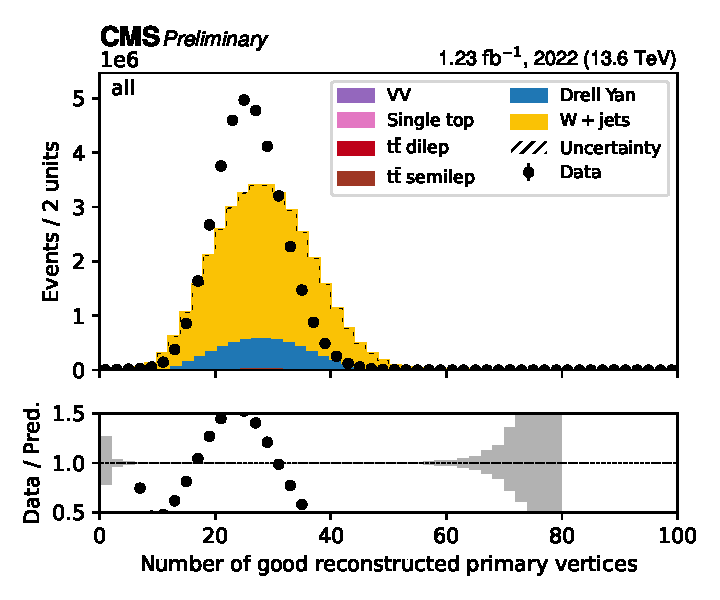
\includegraphics[width=0.49 \textwidth]{figures/ttxs/pileup/nvtx_orig.pdf}
    \hfill
    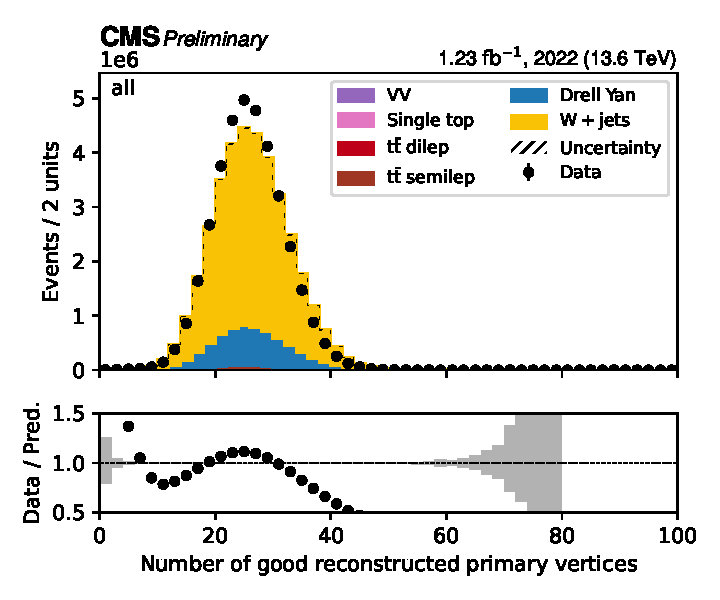
\includegraphics[width=0.49 \textwidth]{figures/ttxs/pileup/nvtx_reweighted.pdf}
    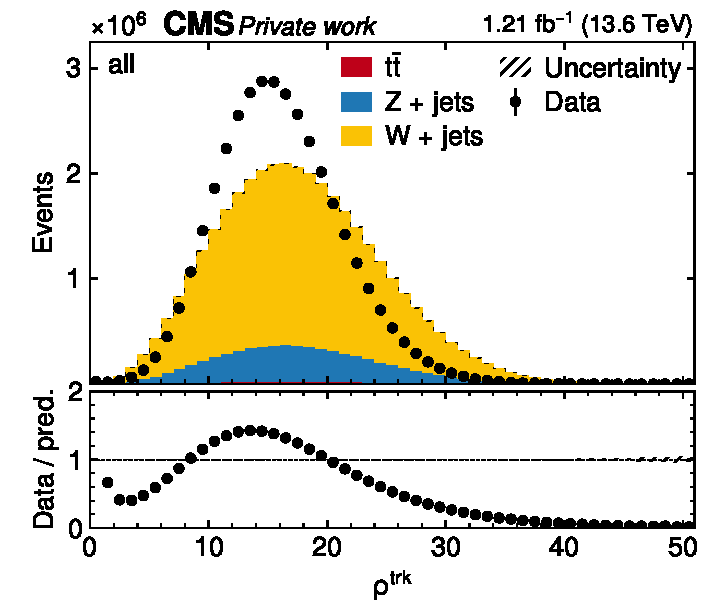
\includegraphics[width=0.49 \textwidth]{figures/ttxs/pileup/rhoFastjetCentralChargedPileUp_orig.pdf}
    \hfill
    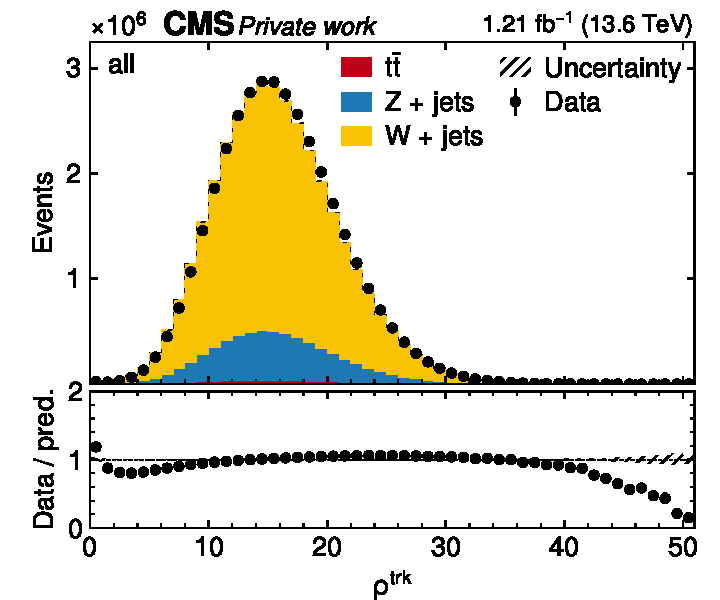
\includegraphics[width=0.49 \textwidth]{figures/ttxs/pileup/rhoFastjetCentralChargedPileUp_reweighted.pdf}
    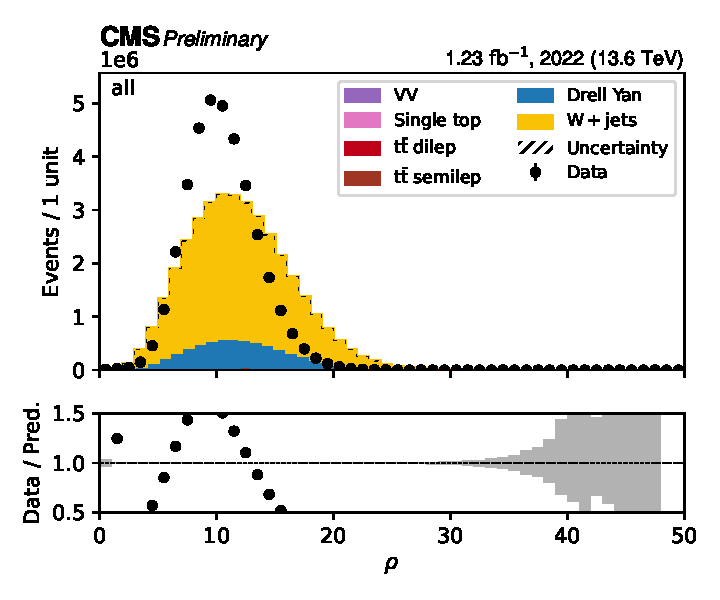
\includegraphics[width=0.49 \textwidth]{figures/ttxs/pileup/rhoFastjetCentralCalo_orig.pdf}
    \hfill
    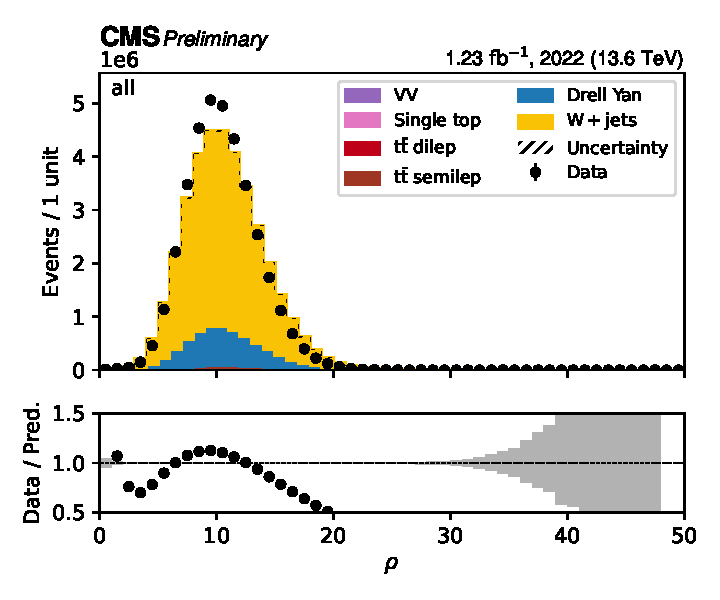
\includegraphics[width=0.49 \textwidth]{figures/ttxs/pileup/rhoFastjetCentralCalo_reweighted.pdf}
    \caption{\textbf{Pileup reweighting.} Pileup-related distributions in MC and data in before (left) and after reweighting (right). From top to bottom: number of primary vertices as well as the mean energy densities $\rho^{\mathrm{calo}}$ (calculated using tracker input) and $\rho^{\mathrm{trk}}$ (calculated using calorimeter input). \todo{prettify plots}}
    \label{fig:ttxs:pileup}
  \end{figure}

\paragraph{Trigger scale factors}

The trigger efficiency, i.e. the probability for an event falling into the selection phase space to be triggered by the low- and high-level triggers, needs to be for in the simulation.
In principle, both dilepton and single-lepton triggers are used for this measurement and should be considered for the efficiency calculation. However, due to the high offline \pt requirements for the two leptons applied in all channels, the fraction of events that are triggered by the dilepton triggers only is very small, and can be neglected for the purpose of determining the scale factor. Thus, only the single-lepton triggers are considered in this section for simplicity.
%It should be noted that, while both dilepton and single-lepton triggers are used for the measurement, the single-lepton triggers by far dominate the selected event count due to the high \pt thresholds required, and so the efficiency is measured for the single-lepton triggers only for simplicity.

The efficiency measurement is performed by the so-called tag-and-probe (T\&P) method, using $\mathrm{Z} \rightarrow \mathrm{e^+ e^-}$ and $\mathrm{Z} \rightarrow \mathrm{\mu^+ \mu^-}$ events. They are selected using the same definitions presented above, including the lepton identification, except for requiring their invariant mass to fulfill $| \mll - m_Z | < 20$ GeV. At least one of the leptons is required to pass the relevant single-lepton trigger and is then designated the tag, while the other lepton might or might not pass the trigger and is designated the probe. Assuming the probability for the two leptons to pass the trigger to be independent of each other, the trigger efficiency, given by probability of the probe to pass, can be written as

\begin{equation}
    \epsilon_{\mathrm{tr}} = \frac{N (\text{Probe passes})}{ N (\text{Probe passes}) + \frac{1}{2} N (\text{Probe fails}) }
\end{equation}

where $N$ is the observed event yield, and the combinatoric factor $\frac{1}{2}$ comes from the fact that either one or the other lepton can fail to pass the trigger. 

The efficiency is measured in this way in coarse bins of lepton \pt and \abseta, seperately for muons and electrons, in both simulation and experimental data. It is then applied to simulation in the following way: For \ljets events, a simple ratio $\epsilon_{\mathrm{tr,data}} / \epsilon_{\mathrm{tr,sim}}$ is applied to each simulation event as a scale factor, which is displayed in \cref{fig:ttxs:triggersf}. For dilepton events, on the other hand, the fact only one lepton needs to pass the single-lepton trigger needs to be taken into account. This leads to a per-event efficiency given by

\begin{equation}
\label{eq:ttxs:triggersf}
    \epsilon_{\mathrm{tr,\ell \ell}} = \epsilon_{\mathrm{tr,\ell 1}} + \epsilon_{\mathrm{tr,\ell 2}} - \epsilon_{\mathrm{tr,\ell 1}} \epsilon_{\mathrm{tr,\ell 2}}
\end{equation}

where $\epsilon_{\mathrm{tr,\ell 1}}$ and $\epsilon_{\mathrm{tr,\ell 2}}$ are the efficiencies evaluated at the \pt and \abseta of the two leptons, respectively. Again, the ratio of this event efficiency in data and simulation is applied to the simulation.

\begin{figure}[t]
    \centering
    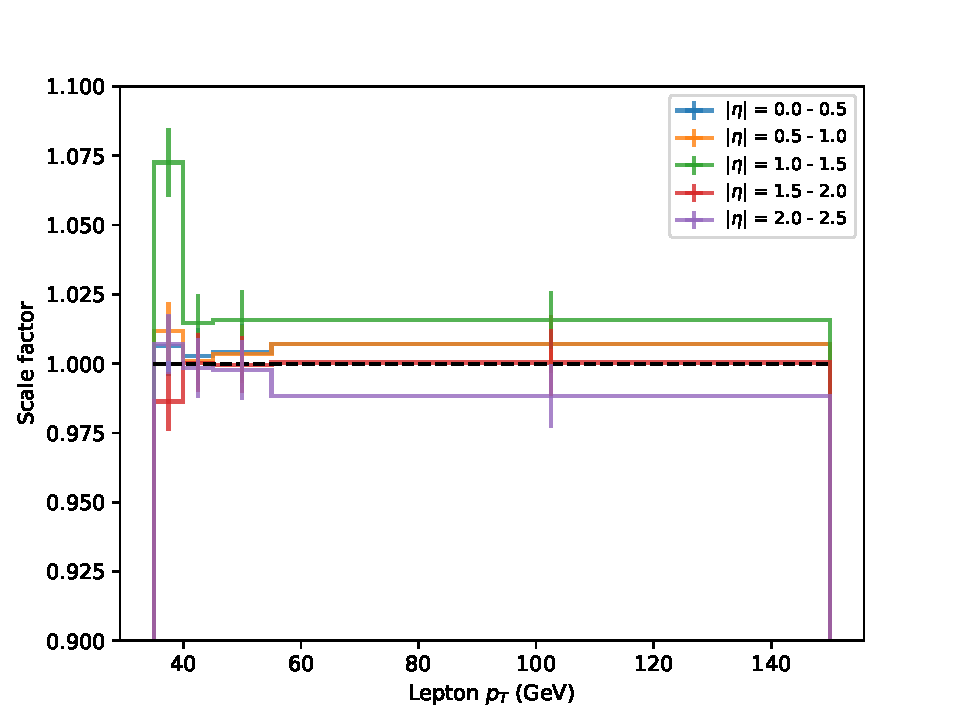
\includegraphics[width=0.49 \textwidth]{figures/ttxs/scalefactors/triggersf_ele.pdf}
    \hfill
    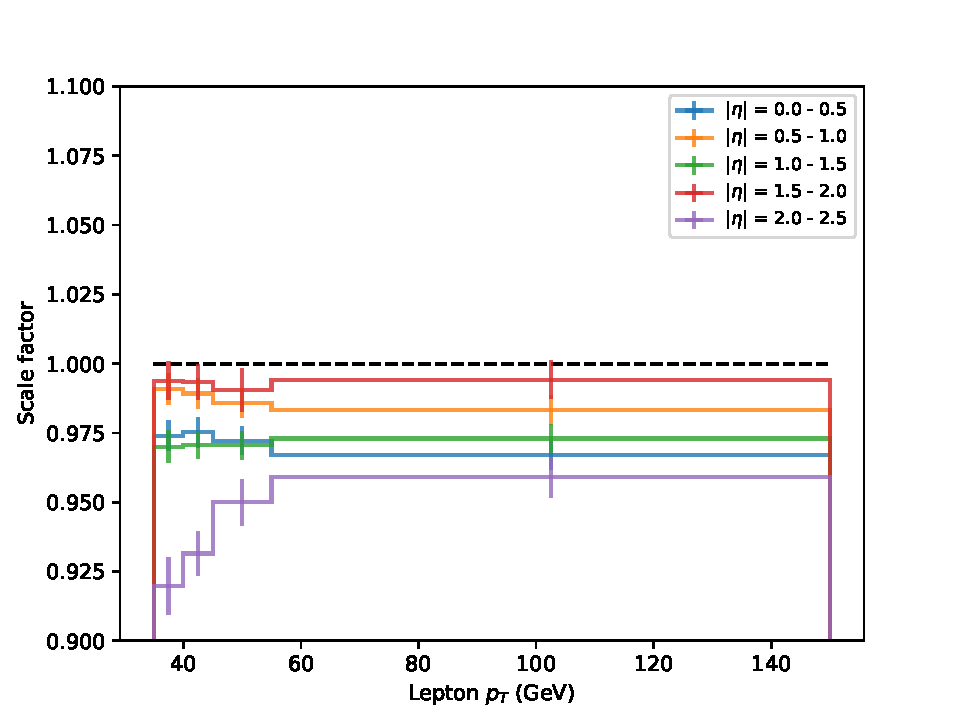
\includegraphics[width=0.49 \textwidth]{figures/ttxs/scalefactors/triggersf_muon.pdf}
    \caption{\textbf{Trigger scale factors.} Single-lepton trigger scale factors for electrons (left) and muons (right) as a function of lepton \pt and $|\eta|$, calculated using a tag-and-probe-method. The error bars designate both statistical and systematic uncertainties. \todo{prettify plots}}
    \label{fig:ttxs:triggersf}
\end{figure}

\paragraph{Lepton scale factors}

Similarly to the triggers, the reconstruction and identification of leptons can exhibit different efficiencies between simulation and data, and thus require scale factors.
%Two orthogonal approaches are taken with respect to this: In the first approach, 
The efficiencies are measured with a similar tag-and-probe method as for the triggers, and the simulation is corrected to the data. This is the standard approach commonly taken in CMS, detailed in \citeres{CMS:EGM-17-001,CMS:MUO-16-001} for electrons and muons, respectively.%, and will be used in the figures presented in this thesis unless stated otherwise. 
The efficiency measurement was not performed as part of this thesis, but is still shown in \cref{fig:ttxs:muonsf,fig:ttxs:elesf} for reference. The muon scale factors are split into a reconstruction and an identification part, while these are combined for the electron scale factors.  

\begin{figure}[t]
    \centering
    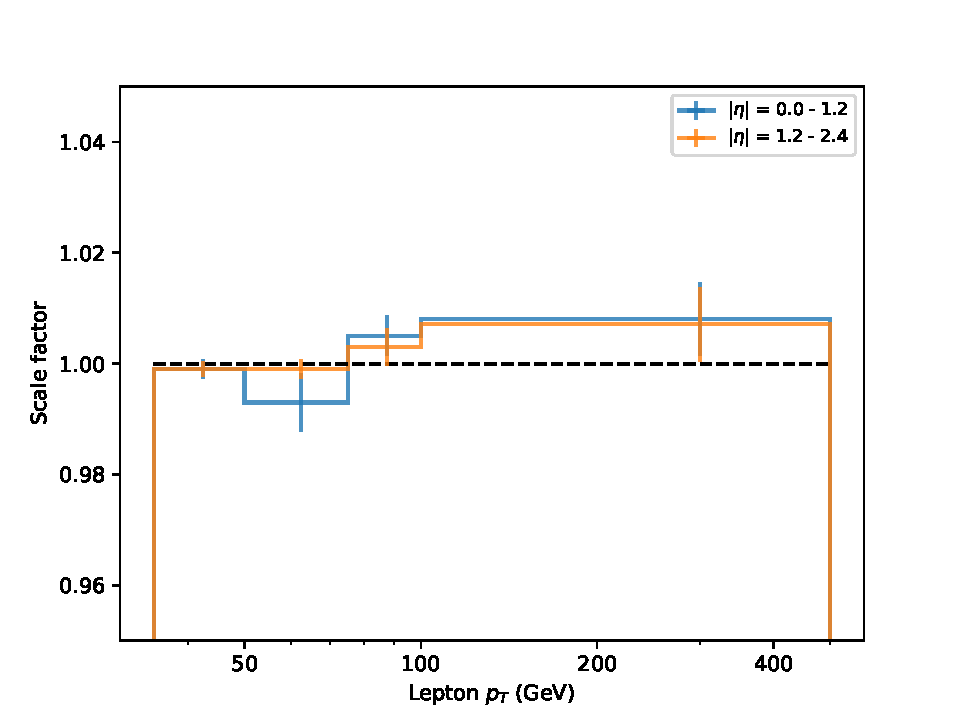
\includegraphics[width=0.49 \textwidth]{figures/ttxs/scalefactors/muonsf_reco.pdf}
    \hfill
    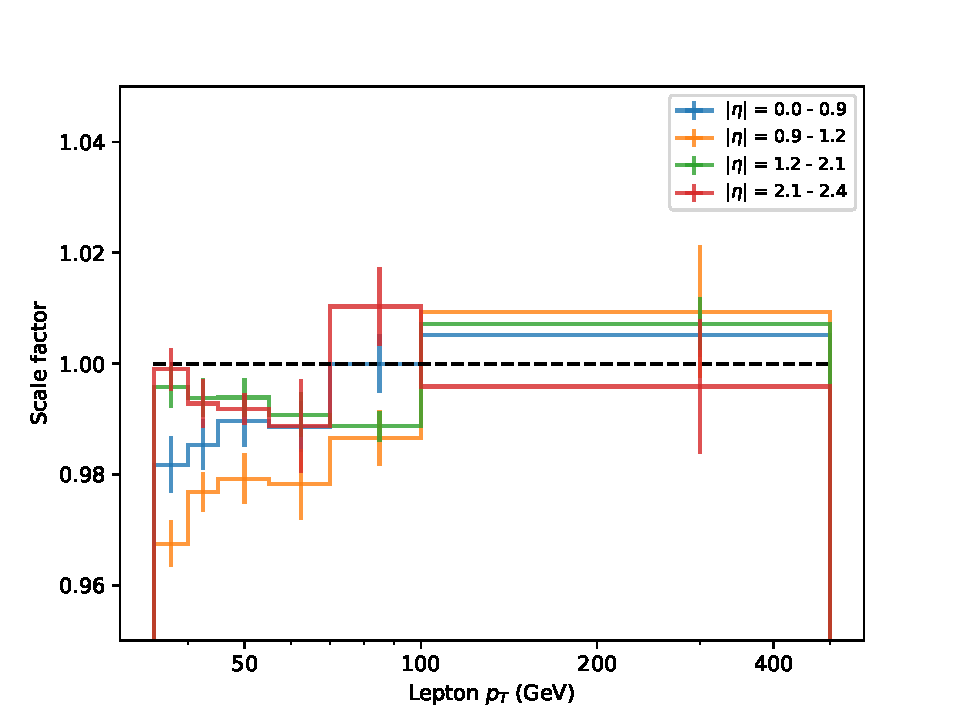
\includegraphics[width=0.49 \textwidth]{figures/ttxs/scalefactors/muonsf_id.pdf}
    \caption{\textbf{Muon scale factors.} They are split into reconstruction (left) and identification (right) and shown as a function of lepton \pt and $|\eta|$, calculated using a tag-and-probe-method. The error bars designate both statistical and systematic uncertainties. \todo{prettify plots}}
    \label{fig:ttxs:muonsf}
  \end{figure}
  
  \begin{figure}[t]
    \centering
    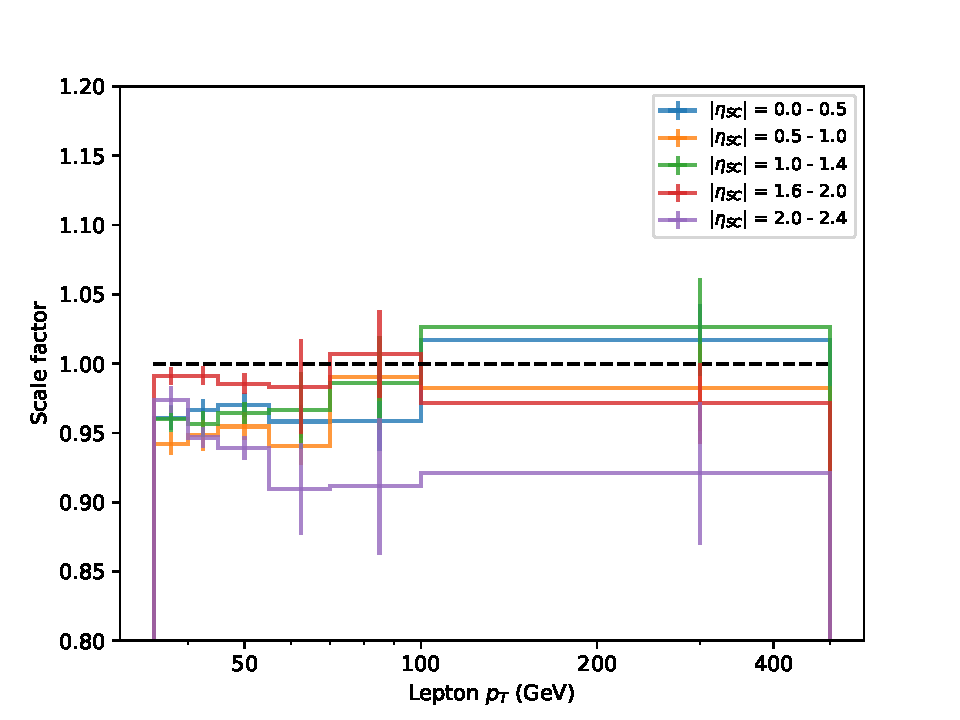
\includegraphics[width=0.49 \textwidth]{figures/ttxs/scalefactors/elesf.pdf}
    \caption{\textbf{Electron scale factors.} The combined electron scale factors as a function of lepton \pt and $|\eta|$, calculated using a tag-and-probe-method. The error bars designate both statistical and systematic uncertainties. \todo{prettify plots}}
    \label{fig:ttxs:elesf}
  \end{figure}

%In the second, alternative, approach, on the other hand, no correction to the simulation is made, and instead the lepton efficiencies in data in the selection phase space are measured simultaneously with the cross section using the likelihood fit. This will be further described in sec. ??.

\paragraph{b tagging scale factors}

The performance of b tagging algorithms, including the \textsc{DeepJet} algorithm used here, is also well-known to have differences between simulation and data, and will need correction factors. This is especially true since the multivariate classifier underlying \textsc{DeepJet} had at the time of the measurement not been re-trained on Run 3 data, and the calibration from Run 2 was used instead.

No external calibration of the b tagging was available at the timescale of this work. Instead, the b tagging efficiency in data will be measured simultaneously with the \ttbar cross section in a single likelihood fit, which is described in more detail in \cref{sec:ttxs:systematics}. No b tagging scale factors are applied at the level of object selection.

\paragraph{Jet energy corrections.}

Another observable that often differs significantly between observed data and simulation is the measured energy response of the jets. It is usually corrected both by theoretical means, e.g. accounting for detector resolution, and by empirical methods, i.e. comparing simulation to data for well-known resonances like the Z boson. The jet energy correction (JEC) is not measured as part of this thesis, and instead centrally provided by CMS following the methods of \citere{CMS:JME-13-004}. 


\subsection{Data-driven background estimation}
\label{sec:ttxs:datadriven}

\paragraph{QCD background}

A significant background contribution in the \ljets channels, especially in the categories with only one b tag, is given by QCD multijet events with one reconstructed lepton. The lepton in question might be non-prompt, meaning from radiation or hadronization, or it might be fake, i.e. a different particle (such as a photon or pion in the case of electrons) misidentified as a lepton.

It is often not practical to estimate this background using MC simulation as is done for the other backgrounds in this analysis. The reason is that, due to the large cross section of QCD multijet events at the LHC but low ratio of events with a fake or non-prompt lepton, very large MC datasets are needed to achieve significant statistics in the selected phase space, which would require excessive computing power. In addition to that, especially fake leptons are not certain to be described well by the simulation.

Instead, a fully data-driven approach is taken to estimate the QCD background in the \ljets channels. For this, several control regions (CRs) orthogonal to the signal region (SR) are defined. In the first CR, denoted ``QCD CR'', the same cuts as in the SR are applied, except that the requirement for the single lepton to be isolated from other particles (see sec. \ref{sec:ttxs:objects}) is inverted. It is expected that QCD events that fall in either the QCD CR or the SR show similar shapes in observable distributions, as long as said observables are uncorrelated with the lepton isolation. Thus, the shape of the QCD background can be extracted from the CR and applied in the SR. \cref{fig:ttxs:np_plots_mj_CR,fig:ttxs:np_plots_ej_CR} show some control distributions in the \mujets and \ejets channels, respectively, with the difference between data and MC in this region considered QCD background.

\begin{figure}[!ht]
    \centering
    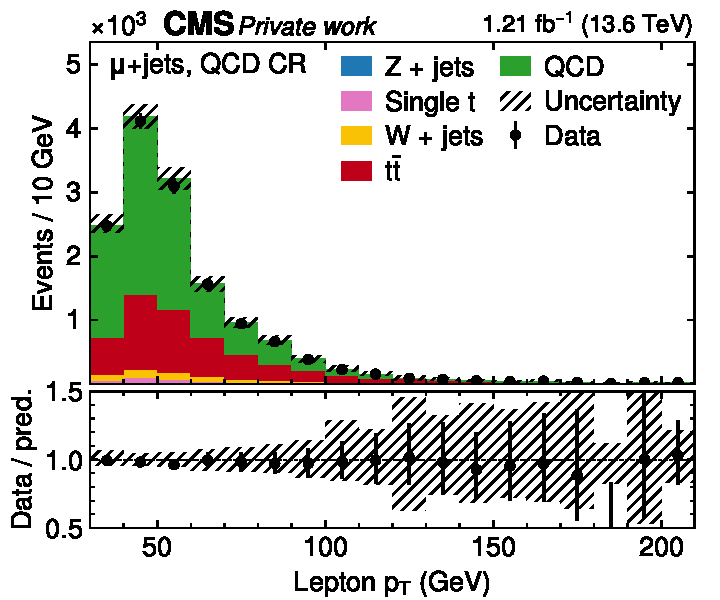
\includegraphics[width=0.49 \textwidth]{figures/ttxs/np_plots_run3/lep_pt_mj_CR.pdf}
    \hfill
    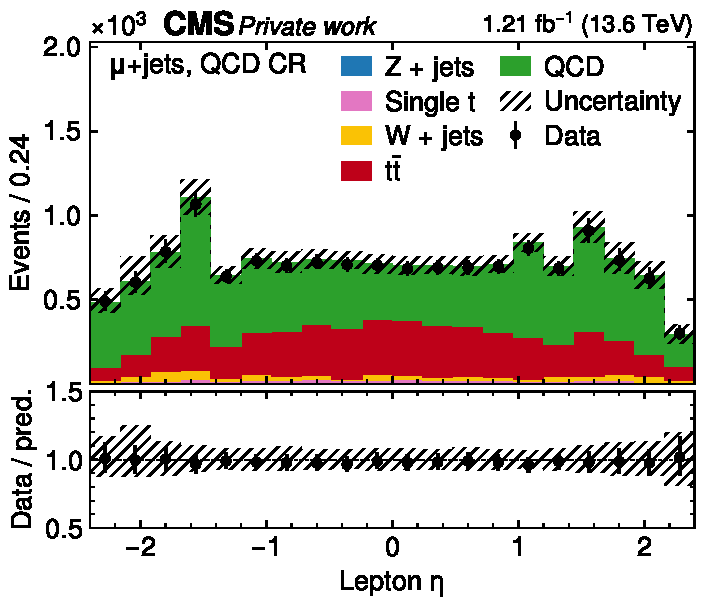
\includegraphics[width=0.49 \textwidth]{figures/ttxs/np_plots_run3/lep_eta_mj_CR.pdf}
    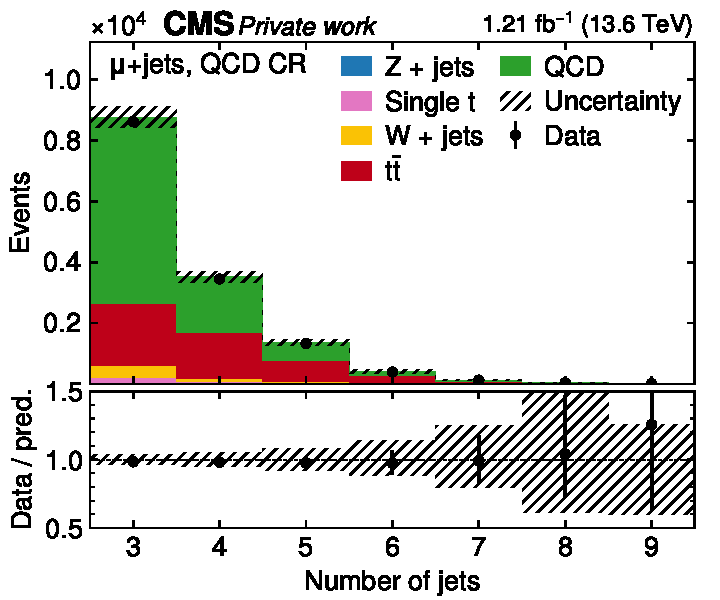
\includegraphics[width=0.49 \textwidth]{figures/ttxs/np_plots_run3/njet_mj_CR.pdf}
    \hfill
    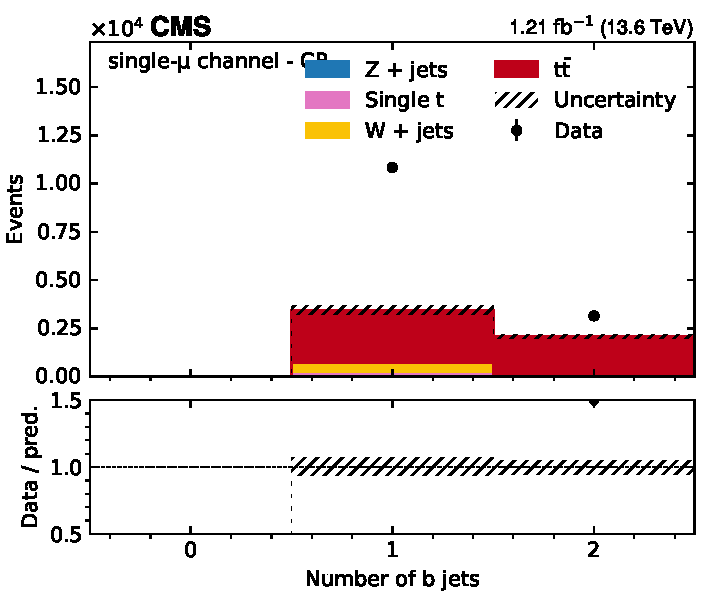
\includegraphics[width=0.49 \textwidth]{figures/ttxs/np_plots_run3/nbtag_mj_CR.pdf}
    \caption{\textbf{QCD control region for \mujets.} Distributions in the QCD CR for the \mujets channel. From top left to bottom right: $\pt$ of the lepton, $\eta$ of the lepton, the number of jets, and the number of b-tagged jets. The uncertainty bands include MC statistical and systematic uncertainties. The difference between data and MC is considered QCD background. \todo{prettify plots; also actually show the estimated QCD in green instead of as the difference between data and MC}}
    \label{fig:ttxs:np_plots_mj_CR}
\end{figure}

\begin{figure}[!ht]
    \centering
    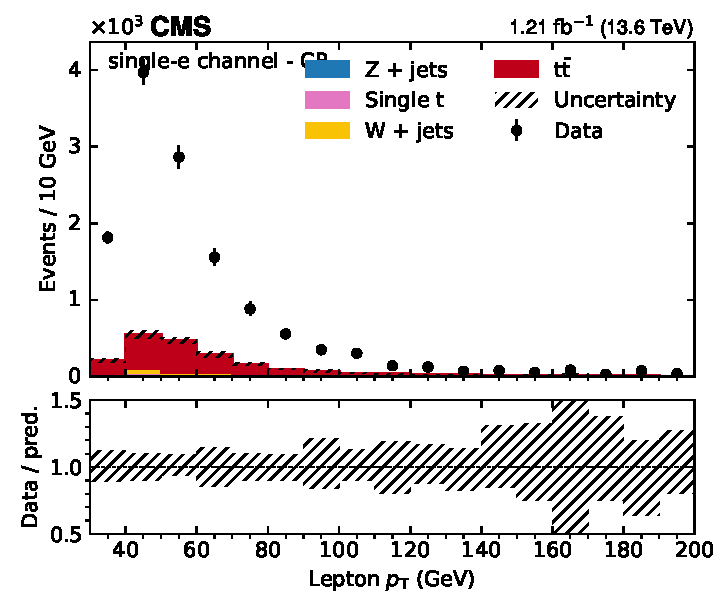
\includegraphics[width=0.49 \textwidth]{figures/ttxs/np_plots_run3/lep_pt_ej_CR.pdf}
    \hfill
    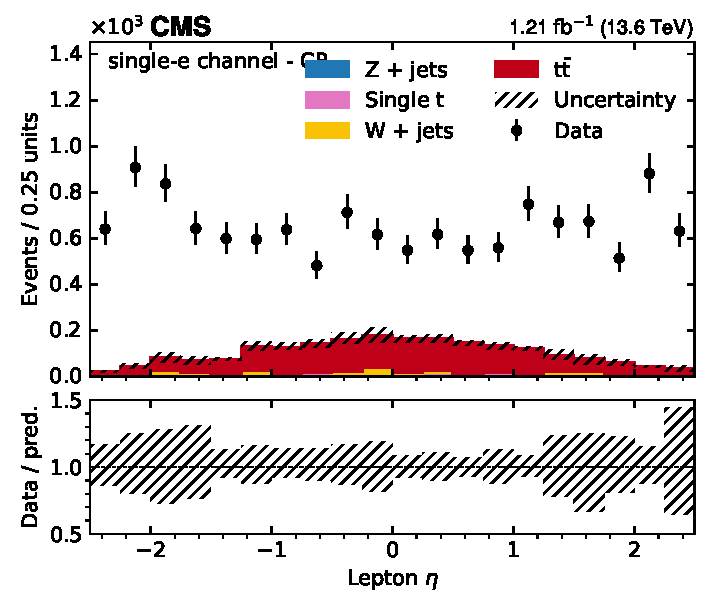
\includegraphics[width=0.49 \textwidth]{figures/ttxs/np_plots_run3/lep_eta_ej_CR.pdf}
    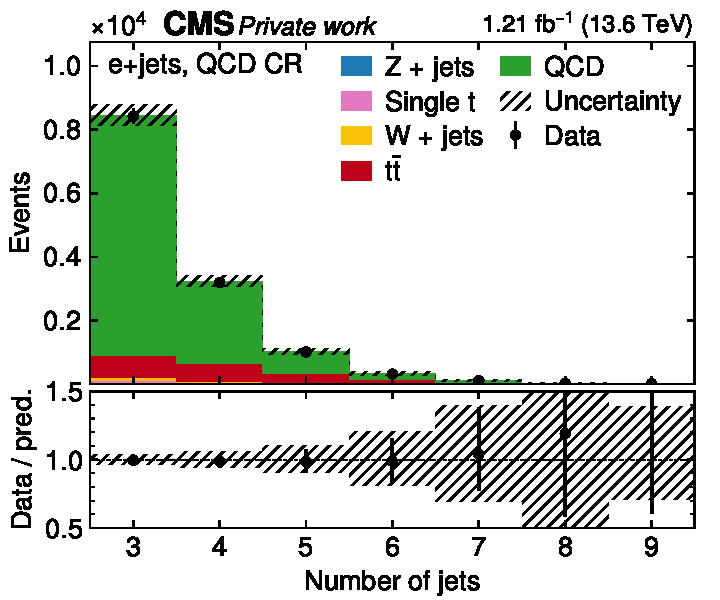
\includegraphics[width=0.49 \textwidth]{figures/ttxs/np_plots_run3/njet_ej_CR.pdf}
    \hfill
    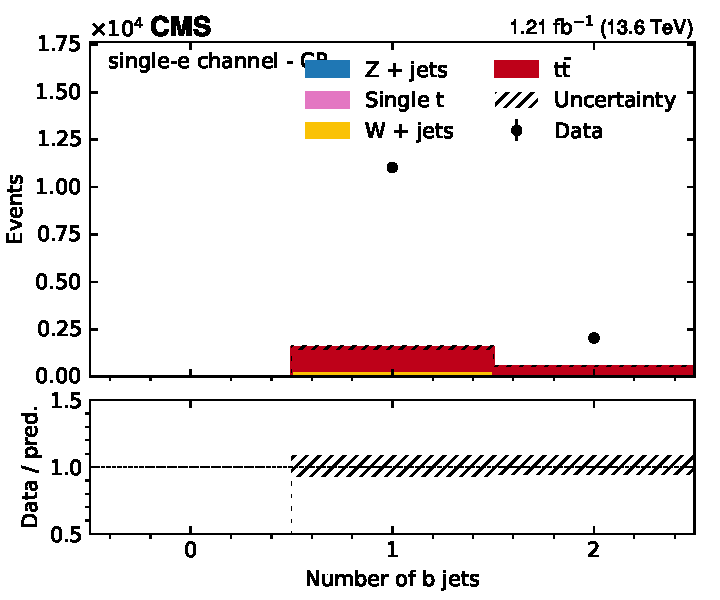
\includegraphics[width=0.49 \textwidth]{figures/ttxs/np_plots_run3/nbtag_ej_CR.pdf}
    \caption{\textbf{QCD control region for \ejets.} Distributions in the QCD CR for the \ejets channel, same as in \cref{fig:ttxs:np_plots_mj_CR}. \todo{prettify plots}}
    \label{fig:ttxs:np_plots_ej_CR}
  \end{figure}

The normalization of the QCD background is fixed through the so-called \textit{ABCD method}, for which an additional CR (the ``1-jet CR'') is defined.
It again contains events that pass the main selection, except for requiring exactly one jet (as opposed to at least three jets in the SR or QCD CR). These events are enriched with QCD events and contain negligible amounts of \ttbar signal. They are used to measure the ratio $f_{\mathrm{fake}}$ of QCD events that pass or fail the lepton isolation requirement, given by

\begin{equation}
\label{eq:ttxs:abcd_fakerate}
    f_{\mathrm{fake}} = \frac{ N_{\text{1 jet, pass}}^{\text{data}} - N_{\text{1 jet, pass}}^{\text{MC}} }{ N_{\text{1 jet, fail}}^{\text{data}} - N_{\text{1 jet, fail}}^{\text{MC}} }
\end{equation}

where $N_{\text{1 jet, pass}}$ and $N_{\text{1 jet, fail}}$ denote 1-jet-events that pass and fail the lepton isolation requirement, respectively, ``data'' refers to the experimental data, and ``MC'' refers to the sum of all non-QCD processes, which are estimated by MC simulation. Here, this ratio is measured in four coarse bins of lepton \pt and \abseta to accurately model lepton-related distributions; it can be seen in \cref{fig:ttxs:fakerate}.

\begin{figure}[!ht]
    \centering
    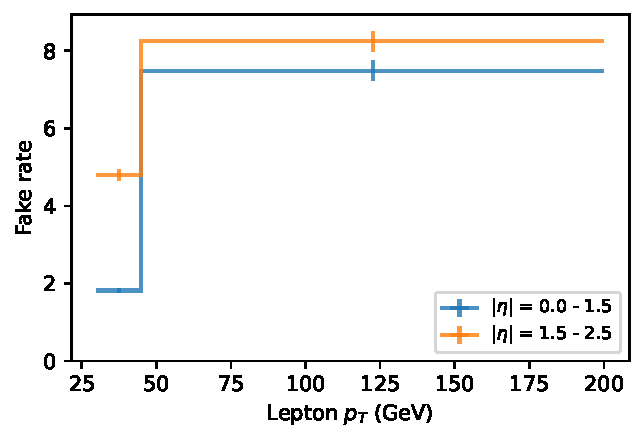
\includegraphics[width=0.49 \textwidth]{figures/ttxs/np_plots_run3/fakerate_eles.pdf}
    \hfill
    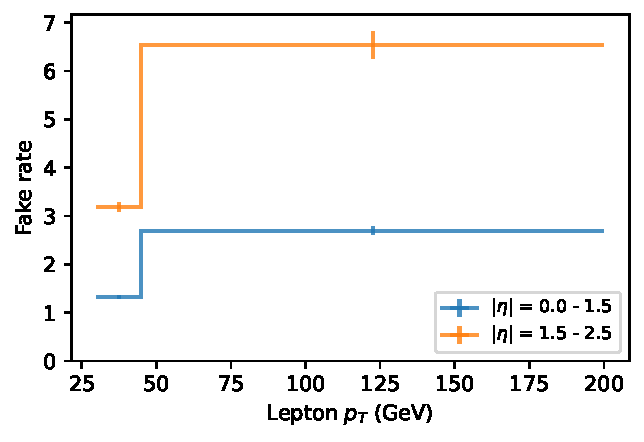
\includegraphics[width=0.49 \textwidth]{figures/ttxs/np_plots_run3/fakerate_muons.pdf}
    \caption{\textbf{QCD fake rate}. The fake rate for the QCD background estimated in the 1 jet bin for electrons (left) and muons (right) as a function of lepton \pt and $|\eta|$. The error bars designate statistical uncertainties only.}
    \label{fig:ttxs:fakerate}
\end{figure}

Naively, the full distribution of the QCD background in the SR for any observable can then be written as

\begin{equation}
\label{eq:ttxs:abcd_naive}
    N_{\text{SR}}^{\text{QCD}} = ( N_{\text{CR}}^{\text{data}} - N_{\text{CR}}^{\text{MC}} ) \times f_{\mathrm{fake}}
\end{equation}

\noindent where $N_{\text{CR}}^{\text{data}}$ and $N_{\text{CR}}^{\text{MC}}$ refer to the total data and non-QCD MC yields in the QCD CR.

In practice, this is complicated by the fact that a non-negligible amount of \ttbar signal is present in the QCD CR, whose cross section, as the parameter of interest in the measurement, is not known \textit{a priori}. %A modified method to correct for this is given in Appendix ??.
To circumvent this problem, a modified method is introduced, which is agnostic about the prediction for the \ttbar cross section. 
One sets for the SR

\begin{equation}
\label{eq:ttxs:abcd_modified1}
    N^{\mathrm{data}}_{\mathrm{SR}} = N^{\ttbar}_{\mathrm{SR}}+ N^{\mathrm{MC,BG}}_{\mathrm{SR}} + N^{\mathrm{QCD}}_{\mathrm{SR}}
\end{equation}

\noindent and similarly for the QCD CR

\begin{equation}
\label{eq:ttxs:abcd_modified2}
    N^{\mathrm{data}}_{\mathrm{CR}} = N^{\ttbar}_{\mathrm{CR}} + N^{\mathrm{MC,BG}}_{\mathrm{CR}} + N^{\mathrm{QCD}}_{\mathrm{CR}},
\end{equation}

\noindent where $N^{\mathrm{data}}$ is the total data yield, $N^{\ttbar}$ is the \ttbar signal contribution, $N^{\mathrm{MC,BG}}$ is the contribution of non-QCD backgrounds as predicted by MC, and $N^{\mathrm{QCD}}$ is the QCD contribution. It is assumed that the ratio $f_{\mathrm{sig}}$ of signal events in the SR and QCD CR (but not necessarily the normalization) is correctly predicted by MC:

\begin{equation}
\label{eq:ttxs:abcd_modified3}
    f_{\mathrm{sig}} := \frac{ N^{\ttbar}_{\mathrm{CR}} }{ N^{\ttbar}_{\mathrm{SR}} } = \frac{ N^{\mathrm{\ttbar,MC}}_{\mathrm{CR}} }{ N^{\mathrm{\ttbar,MC}}_{\mathrm{SR}} }
\end{equation}

Furthermore, one sets similar to \cref{eq:ttxs:abcd_naive}

\begin{equation}
\label{eq:ttxs:abcd_modified4}
    N^{\mathrm{QCD}}_{\mathrm{SR}} = N^{\mathrm{QCD}}_{\mathrm{CR}} \times f_{\mathrm{fake}}
\end{equation}

\noindent where $f_{\mathrm{fake}}$ is still given by \cref{eq:ttxs:abcd_fakerate}, which is unaffected since the \ttbar signal contamination in the 1-jet CR is negligible.

Combining all these equations, one can first replace $N^{\ttbar}_{\mathrm{CR}}$ in \cref{eq:ttxs:abcd_modified2} by $f_{\mathrm{sig}} N^{\ttbar}_{\mathrm{SR}}$ according to \cref{eq:ttxs:abcd_modified3}, then eliminate $N^{\ttbar}_{\mathrm{SR}}$ in favour of $N^{\mathrm{data}}_{\mathrm{SR}}$, i.e. the total data yield in the SR, and get

\begin{equation}
    N^{\mathrm{QCD}}_{\mathrm{SR}} = f_{\mathrm{fake}} \, \left( N^{\mathrm{data}}_{\mathrm{CR}} - N^{\mathrm{MC,BG}}_{\mathrm{CR}} - f_{\mathrm{sig}} \left( N^{\mathrm{data}}_{\mathrm{SR}} - N^{\mathrm{MC,BG}}_{\mathrm{SR}} - N^{\mathrm{QCD}}_{\mathrm{SR}} \right) \right) .
\end{equation}

Solving this equation for $N^{\mathrm{QCD}}_{\mathrm{SR}}$ finally yields the corrected QCD contribution in the SR:

\begin{equation}
\label{eq:ttxs:abcd_modified}
    N^{\mathrm{QCD}}_{\mathrm{SR}} = \left( N^{\mathrm{data}}_{\mathrm{CR}} - N^{\mathrm{MC,BG}}_{\mathrm{CR}} - f_{\mathrm{sig}} ( N^{\mathrm{data}}_{\mathrm{SR}} - N^{\mathrm{MC,BG}}_{\mathrm{SR}} )\right)
    \times \frac{ f_{\mathrm{fake}} } {1 - f_{\mathrm{sig}} f_{\mathrm{fake}}}
\end{equation}

The resulting QCD distributions from this method are further treated in the same way as the MC backgrounds, and can be seen together with them in \cref{fig:ttxs:control_em,fig:ttxs:control_eemm,fig:ttxs:control_ljets}.
  

\paragraph{Z+jets background}

In contrast to the QCD background, the Z+jets background, which is relevant mostly in the \ee and \mumu channels, can in general be well described by MC simulation. However, in the phase space used in the analysis, there can be problems related to the b tag requirement. For Z+jets events, b jets are only generated at the matrix element level at higher orders in perturbative QCD, and might thus not be well modeled compared to observed data. This in turn could influence the acceptance of Z+jets events, leading to an incorrect normalization in events with one or more b tags.

Here, a data-driven normalization is derived for Z+jets events with one or two b tags in the dilepton channels, following \citere{CMS:EXO-22-014-PAS}. This is important especially in the same-flavor channels, where Z+jets is a dominant background.

The normalization is derived using a CR in which the cut on \mll is inverted, i.e. in events with $| \mll - m_Z | < 15$ GeV ("inside the Z window"), which are strongly enriched in Z+jets contributions. It is assumed that the Z+jets contribution in the \emu channel (which stems mostly from $\mathrm{Z} \rightarrow \tau \tau$ events) is negligible compared to the ee and $\mu \mu$ channels, and that all other backgrounds (including \ttbar) are approximately equal in the three dilepton channels up to combinatorics, in the sense that their differences are small compared to the Z+jets event yield. Then, said Z+jets yield in the Z window in the same-flavor channels can be estimated directly from data by subtracting the \emu channel -- and with it, the other backgrounds - from the \ee and \mumu channels. This results in

\begin{equation}
\label{eq:ttxs:zjets_yield}
    N_{\mathrm{ee / \mu\mu}}^{\mathrm{Z+jets}} = N_{\mathrm{ee / \mu\mu,\,in}}^{\mathrm{data}} - \frac{1}{2} N_{\mathrm{\emu,\,in}}^{\mathrm{data}} \, k_{\mathrm{ee / \mu\mu,\,in}}
\end{equation}

\noindent where $N_{\mathrm{\ell \ell},\,in}^{\mathrm{data}}$ refers to the number of observed events inside the Z window for the respective channel, and $k_{\mathrm{ee}} = k_{\mathrm{\mu\mu}}^{-1} = \sqrt{N_{\mathrm{ee,\,in}}^{\mathrm{data}} / N_{\mathrm{\mu\mu,\,in}}^{\mathrm{data}}}$ is a efficiency factor to correct for the different acceptance of electrons and muons.

To translate this yield from the CR to the SR, the ratio $\Rinout = N_{\mathrm{in}}^{\mathrm{Z+jets}} / N_{\mathrm{out}}^{\mathrm{Z+jets}}$ (referring to \textit{inside} and \textit{outside} of the Z window) of event numbers between those two regions has to be estimated. This could in principle be done by directly using the MC simulation (as done in e.g. \citeres{CMS:EXO-16-049,CMS:HIG-17-027}). However, since this ratio might by itself be mismodeled in MC, a more cautious approach is taken here. A second CR is defined from events with 0 b tags (which are not considered in the main measurement in the same-flavor channels) and used to construct to construct a more loose assumption:

\begin{equation}
    \frac{  \Rinout^{\text{data}} ( \geq \text{1 b tag} ) } { \Rinout^{\text{MC}} ( \geq \text{1 b tag} ) } = \frac{  \Rinout^{\text{data}} ( \text{0 b tags} ) } { \Rinout^{\text{MC}} ( \text{0 b tags} ) }
\end{equation}

This equation means that the \textit{ratio of ratios} $\Rinout( \geq \text{1 b tag} ) / \Rinout( \text{0 b tags} )$ is assumed to be well described by MC.
It can be solved for the Z+jets yield outside of the Z window in the same-flavor channels, yielding

\begin{equation}
\begin{split}
    N_{\mathrm{out}}^{\mathrm{Z+jets}} &= \frac {N_{\mathrm{in}}^{\mathrm{Z+jets}}} {\Rinout^{\text{data}} ( \geq \text{1 b tag} )}  \\
    &= \frac{  \Rinout^{\text{MC}} ( \text{0 b tags} ) } { \Rinout^{\text{data}} ( \text{0 b tags} ) } \, \frac {N_{\mathrm{in}}^{\mathrm{Z+jets}}} {\Rinout^{\text{MC}} ( \geq \text{1 b tag} )}
\end{split}
\end{equation}

\noindent where $N_{\mathrm{in}}^{\mathrm{Z+jets}}$ is given by \cref{eq:ttxs:zjets_yield}. In practice, this yield is quoted  as a scale factor compared to the nominal MC prediction. For the \emu channel (in which Z+jets is much less important), the scale factor is simply assumed to be the geometric mean of the \ee and \mumu scale factors.

\begin{table}[t]
    \begin{centering}
    \begin{tabular}{|c|c|c|}
    \hline
    \ee & \emu & \mumu \tabularnewline
    \hline
    \hline
    $1.36 \pm 0.04$ & $1.32 \pm 0.03$ & $1.28 \pm 0.03$ \\
    \hline
    \end{tabular}
    \par\end{centering}
    \caption{\textbf{Z+jets scale factors.} Ratio of the Z+jets event yields estimated in data using the method described in \cref{sec:ttxs:datadriven} to the prediction by the MC simulation. Uncertainties are statistical only.}
    \label{tab:ttxs:dysf}
\end{table}

The final scale factors can be seen in \cref{tab:ttxs:dysf}.

\section{Control distributions}
\label{sec:ttxs:control}

In this section, the agreement between simulation and data in several control distributions is presented, shown in \cref{fig:ttxs:control_em,fig:ttxs:control_eemm,fig:ttxs:control_ljets}. All corrections described in the previous section are applied in these figures. In addition, they are already scaled by the b tagging scale factors as will be measured in the likelihood fit (\cref{sec:ttxs:fitresults}).

\begin{figure}[!hp]
\centering
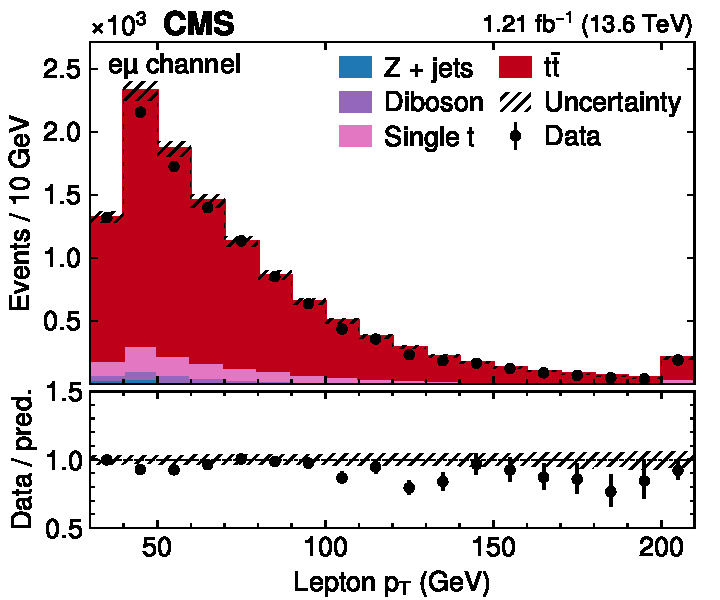
\includegraphics[width=0.49\textwidth]{figures/ttxs/lep_pt_em.pdf}
\hfill
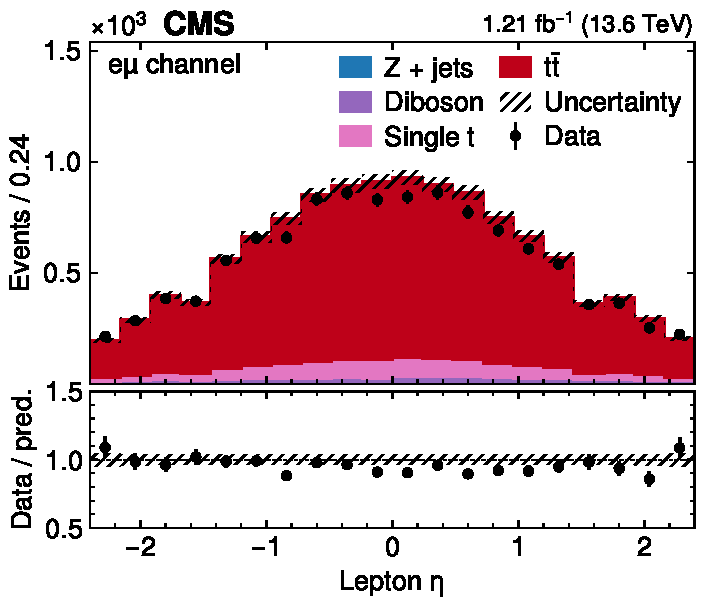
\includegraphics[width=0.49\textwidth]{figures/ttxs/lep_eta_em.pdf}
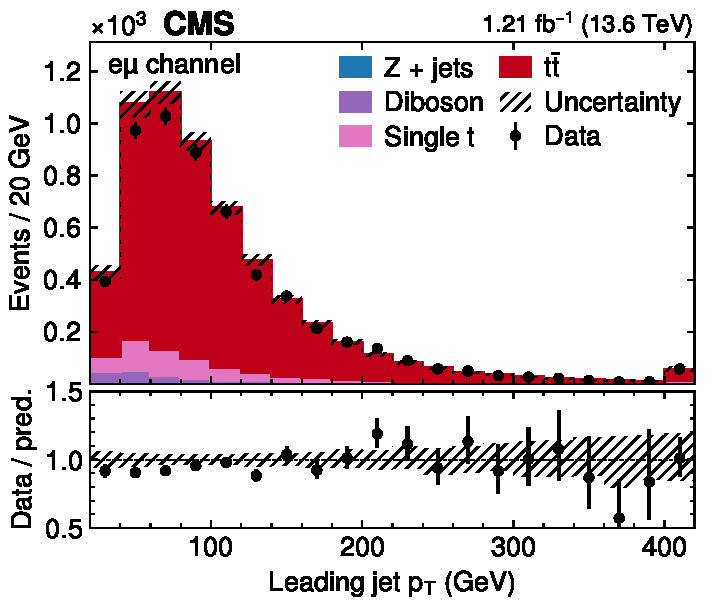
\includegraphics[width=0.49\textwidth]{figures/ttxs/1st_jet_pt_em.pdf}
\hfill
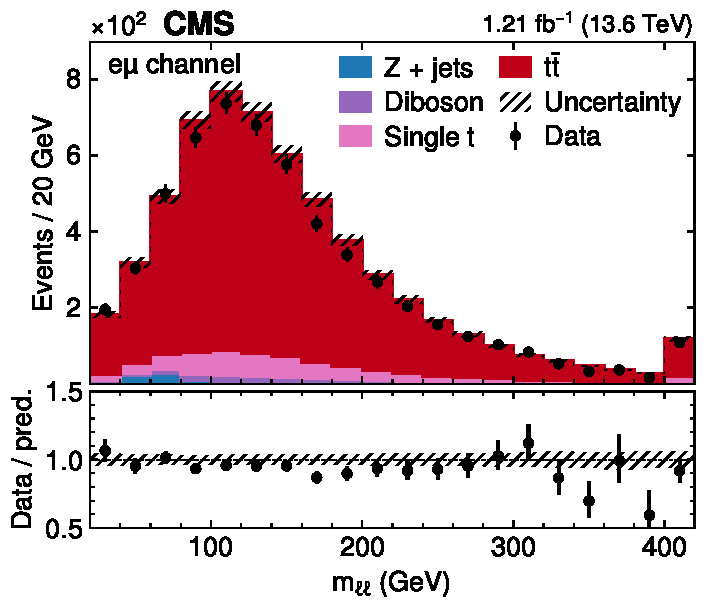
\includegraphics[width=0.49\textwidth]{figures/ttxs/mll_em.pdf}
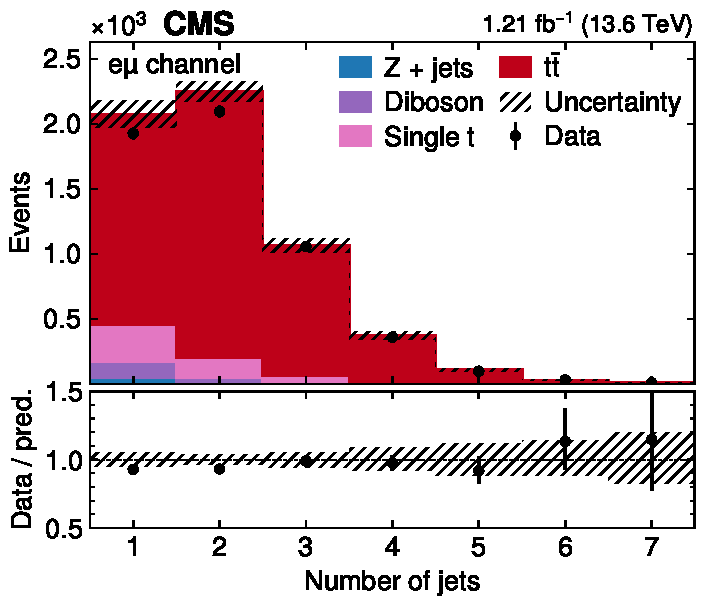
\includegraphics[width=0.49\textwidth]{figures/ttxs/njet_em.pdf}
\hfill
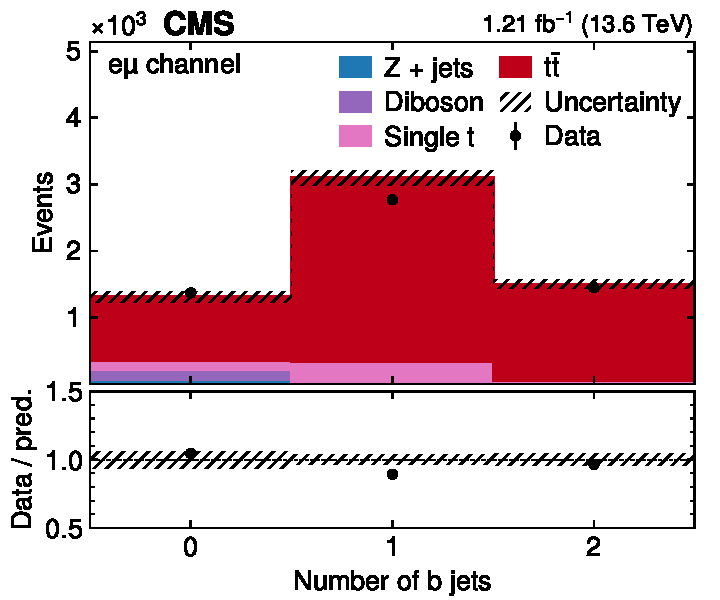
\includegraphics[width=0.49\textwidth]{figures/ttxs/nbtag_em.pdf}
\caption{
    \textbf{Control distributions in the \emu channel.} Shown are (from top left to bottom right) the distributions of \pt of both leptons, \abseta of both leptons, \pt of the leading jet, the invariant lepton mass \mll, the number of jets and the number of b jets. All figures show both data (black dots) and different simulated background processes (colored bars). For the latter, all corrections described in \cref{sec:ttxs:corrections} as well as post-fit b tagging scale factors (\cref{sec:ttxs:fitresults}) are applied, and the shaded area covers both statistical and systematic uncertainties. 
}
\label{fig:ttxs:control_em}
\end{figure}

\begin{figure}[!hp]
\centering
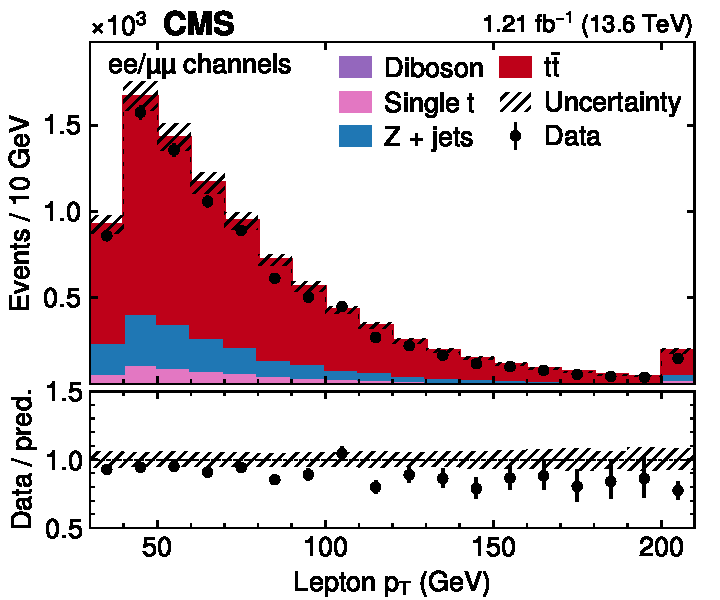
\includegraphics[width=0.49\textwidth]{figures/ttxs/lep_pt_eemm.pdf}
\hfill
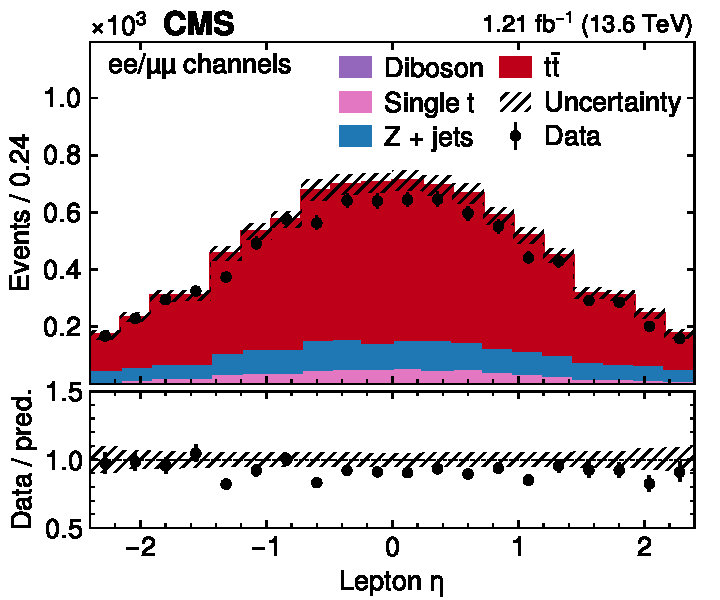
\includegraphics[width=0.49\textwidth]{figures/ttxs/lep_eta_eemm.pdf}
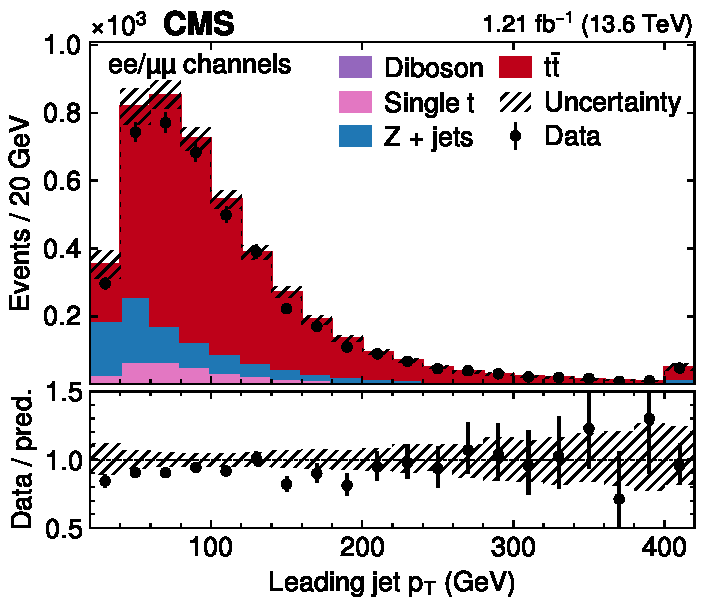
\includegraphics[width=0.49\textwidth]{figures/ttxs/1st_jet_pt_eemm.pdf}
\hfill
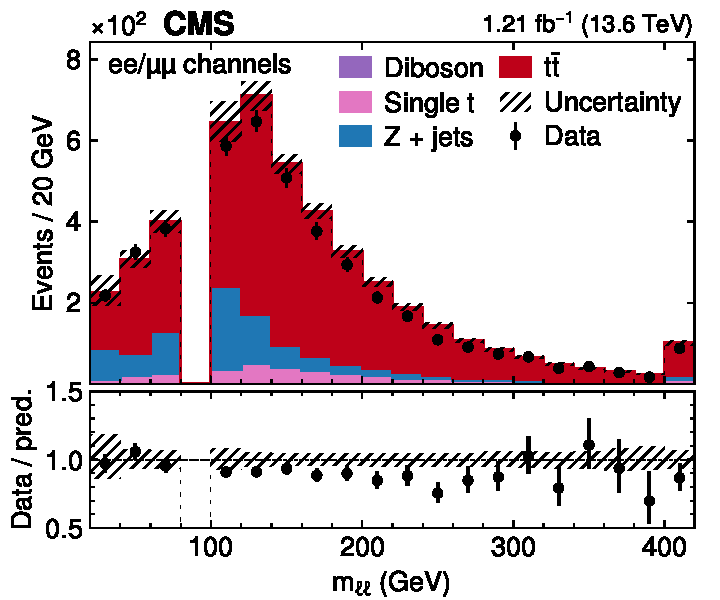
\includegraphics[width=0.49\textwidth]{figures/ttxs/mll_eemm.pdf}
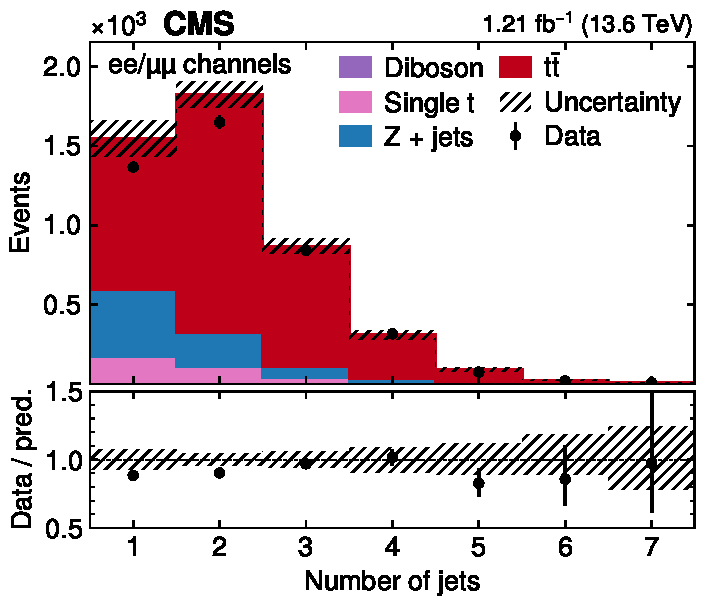
\includegraphics[width=0.49\textwidth]{figures/ttxs/njet_eemm.pdf}
\hfill
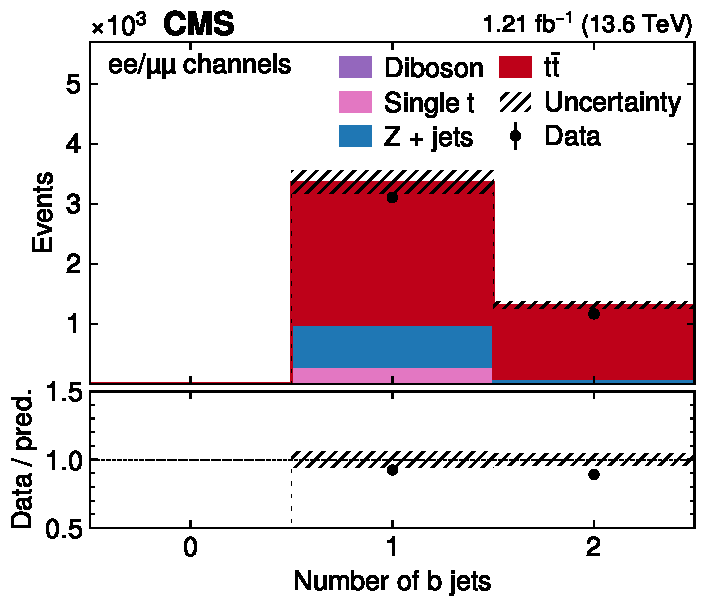
\includegraphics[width=0.49\textwidth]{figures/ttxs/nbtag_eemm.pdf}
\caption{
    \textbf{Control distributions in the \ee and \mumu channels.} The distributions are shown in the same manner as in Fig.~\ref{fig:ttxs:control_em}.
}
\label{fig:ttxs:control_eemm}
\end{figure}

\begin{figure}[!hp]
\centering
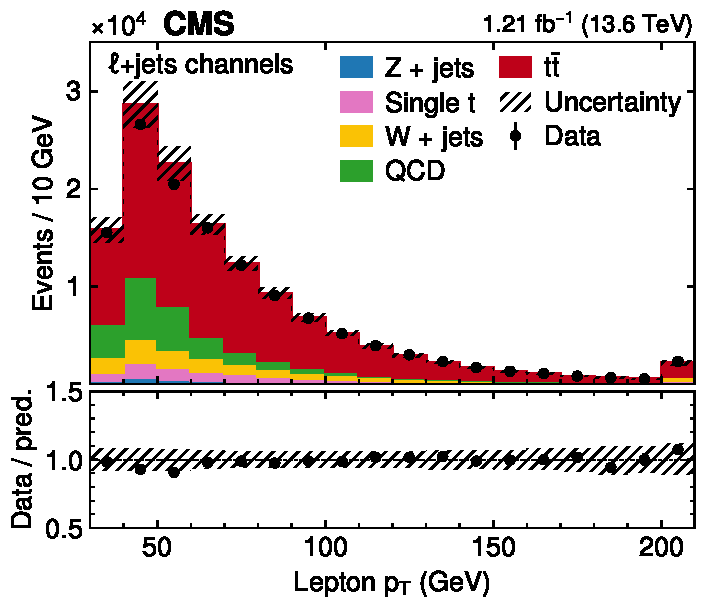
\includegraphics[width=0.49\textwidth]{figures/ttxs/lep_pt_lj.pdf}
\hfill
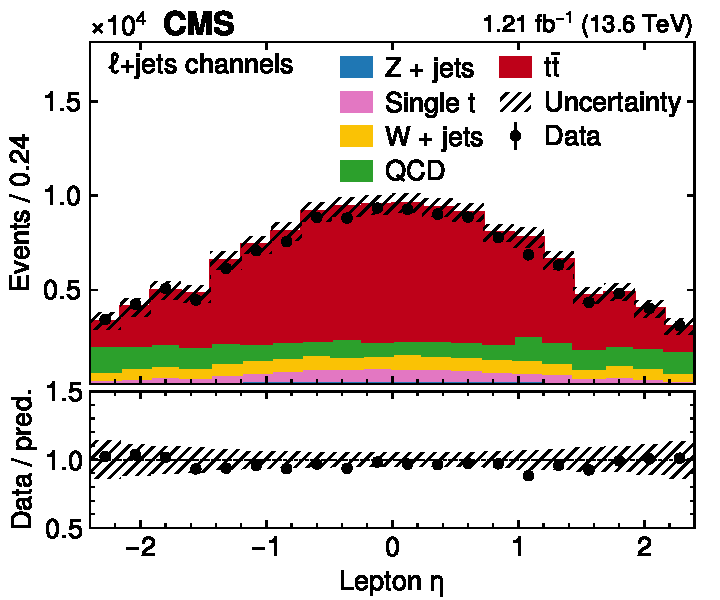
\includegraphics[width=0.49\textwidth]{figures/ttxs/lep_eta_lj.pdf}
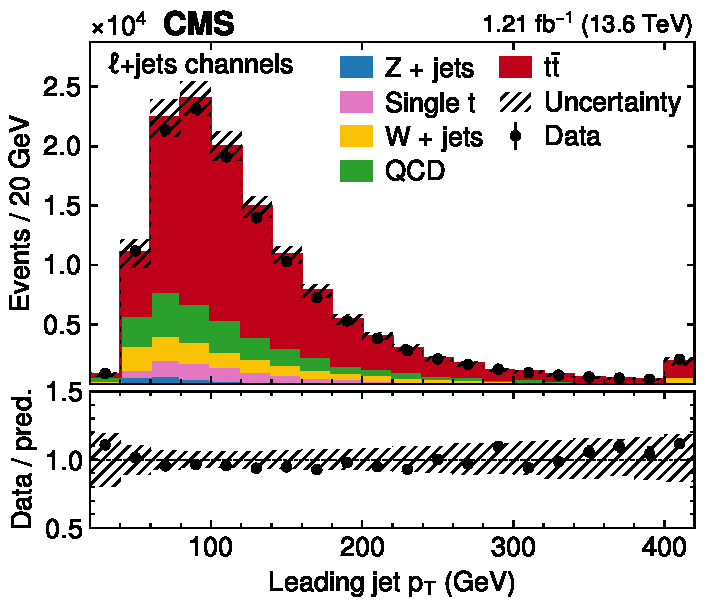
\includegraphics[width=0.49\textwidth]{figures/ttxs/1st_jet_pt_lj.pdf}
\hfill
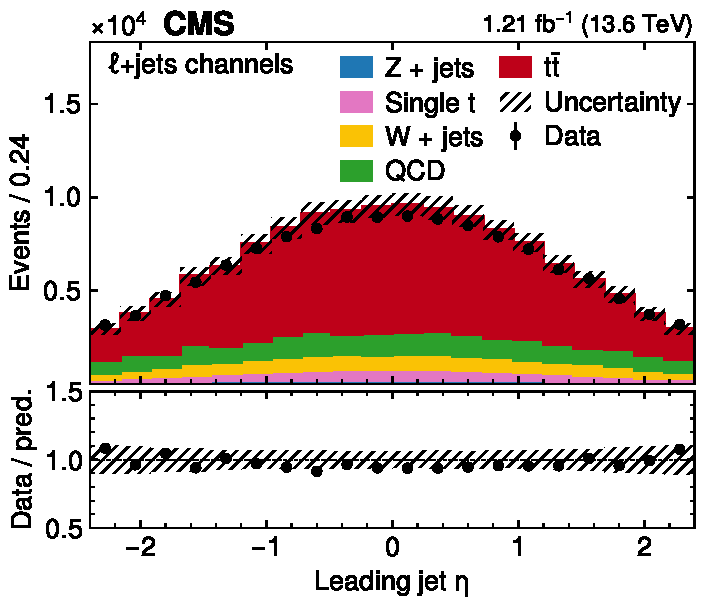
\includegraphics[width=0.49\textwidth]{figures/ttxs/1st_jet_eta_lj.pdf}
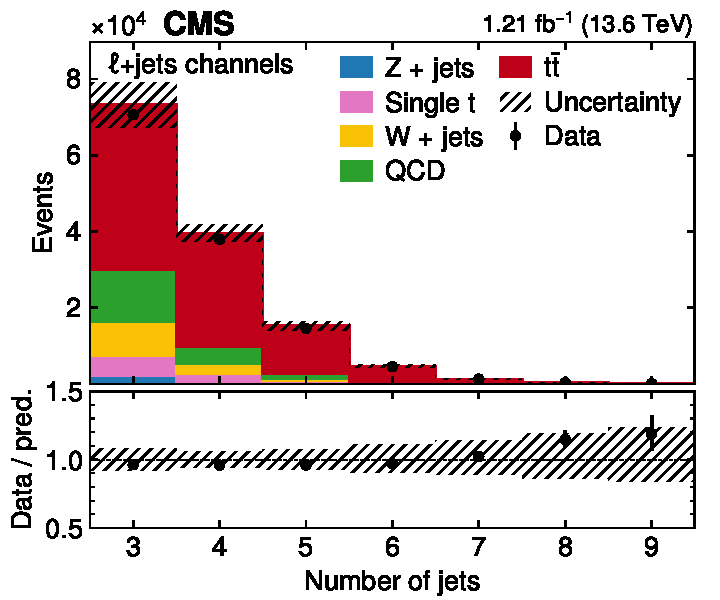
\includegraphics[width=0.49\textwidth]{figures/ttxs/njet_lj.pdf}
\hfill
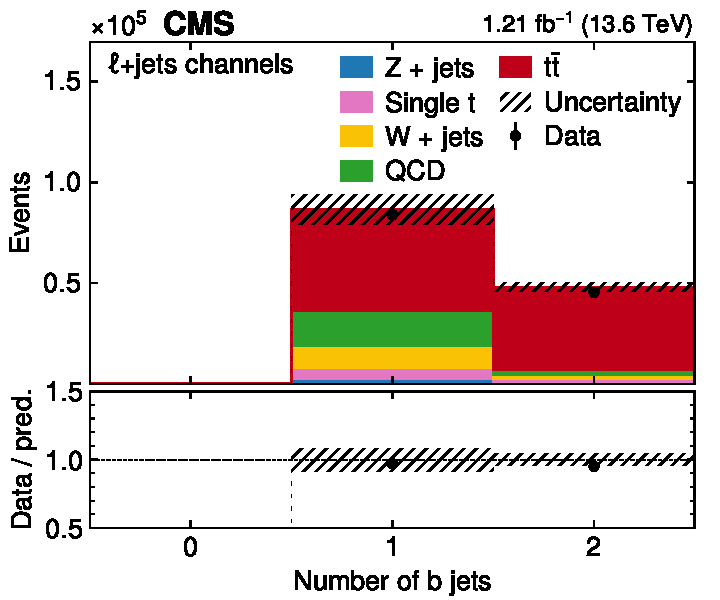
\includegraphics[width=0.49\textwidth]{figures/ttxs/nbtag_lj.pdf}
\caption{
   \textbf{Control distributions in the \ljets channels.} The distributions are shown in the same manner as in Fig.~\ref{fig:ttxs:control_em}, except for the center-right figure, which here shows \abseta of the leading jet.
}
\label{fig:ttxs:control_ljets}
\end{figure}

Good agreement between data and simulation within the full uncertainties is seen in all distributions.

%\section{Likelihood fit}
%\label{sec:ttxs:fit}


\section{Systematic uncertainties}
\label{sec:ttxs:systematics}

% required: general shape uncertainties, special treatment of btag uncertainty, special treatment of lepton uncs in free floating case, XS uncs, lumi unc.

In order to translate the distribution of observed and expected events into a result for the inclusive \ttbar cross section while taking into account all relevant sources of systematic uncertainties, a binned profile maximum likelihood fit as described in \cref{sec:methods:stat} is performed using the tool \texttt{combine}~\cite{CMS:CAT-23-001}.
The parameter of interest (POI) used for this fit is the signal strength $r = \sigmatt / \sigmatt^{\text{pred}}$, i.e. the inclusive \ttbar cross section normalized to its theoretical prediction. A linear signal model is used as defined in \cref{eq:methods:linearsignal}, and the \ttbar cross section is extracted using its maximum likelihood estimate and uncertainty.

This section describes the considered systematic uncertainties, which can be divided into experimental uncertainties, arising from incomplete knowledge of the details of the detector and resulting differences between data and simulation, and theoretical uncertainties, which concern imperfect modeling of the underlying physical processes in the different event generators. All of them will be described in this section.

All systematic uncertainties are included in the fit as nuisance parameters (NPs) as discussed in \cref{sec:methods:stat}. In practice, NPs which encode shape effects on the considered observables are implemented using \textit{template morphing}, i.e. a smooth polynominal interpolation between the nominal shape and the shapes encoding the variations by $\pm 1$ standard deviations. NPs that encode only normalization effects are instead implemented as simple log-normal uncertainties. Both definitions can be found in detail in \citere{CMS:CAT-23-001}.

Special attention is given in this section to some experimental uncertainties which are important to this measurement. This includes the luminosity, which is the dominating uncertainty, as well as 
%the lepton identification and 
the b tagging uncertainties due to the special way they are treated in the fit.

\paragraph{Luminosity uncertainty}

In order to translate event yields, as measured using histograms, into a result on any cross section, the total integrated luminosity is required as a calibration constant. It is immediately clear that any experimental error on the luminosity will be directly transferred to the total error on the measurement, and thus minimizing the luminosity uncertainty is crucial for any cross section mesurement.

For the dataset used in this analysis, the total luminosity uncertainty was evaluated by CMS to be 2.3\%. Of this figure, 2.1\% is due to the calibration of the integrated luminosity, using the methods presented in \citere{CMS:LUM-17-003}. The largest contribution comes from factorization bias, which arises in the van der Meer method from the assumption that the transverse luminous area factorizes in the $x$ and $y$ coordinates, and from residual beam position deviations.

The agreement in the absolute scale is checked by comparing different independently calibrated luminosity measurements, and the integrated luminosity measured with the HF and the silicon pixel detector is found to agree at a level of better than 0.8\%.
Taking additional contributions due to residual differences in the time-stability and linearity between the luminosity detectors into account leads to the full figure of 2.3\%.
A cross-check of the integrated luminosity using the yield of reconstructed Z bosons decaying into pairs of muons~\cite{CMS:DP-2023-003}, corrected for efficiencies and normalized to the fiducial cross section prediction calculated at NNLO with next-to-NNLL corrections applied, shows good agreement as well.\footnote{Since publication of this result, a more precise luminosity measurement for 2022 data has become available in \citere{CMS:LUM-22-001-PAS}.}

In contrast to all other uncertainties described below, the uncertainty in the integrated luminosity is not included in the fit, but treated as an external uncertainty and added in quadrature afterwards, since it is expected to factorize completely from all other uncertainties.
The impact of varying the normalization of the backgrounds estimated from simulation by the integrated luminosity uncertainty was found to be negligible.
% TODO.

\paragraph{b tagging uncertainty}

As mentioned in \cref{sec:ttxs:scalefactors}, the efficiency for correctly identifying a jet originating from a b quark (b tagging) is expected to be different in data and simulation. At the time of this measurement, directly after the start of Run 3, no general-purpose b tagging studies had been available. Thus, the approach adopted here is to consider the b tagging efficiency in data to be completely unknown and measure it concurrently with the cross section in the likelihood fit.

For this purpose, the probability for an event with $n_{\mathrm{jet}}$ selected jets to have $n_{\mathrm{b tag}}$ correctly identified b jets, depending on the assumed b tagging efficiency $\epsilon_b$, is assumed to be a multinomial of the form

\begin{equation}
\label{eq:ttxs:btags}
    P (n_{\mathrm{b tag}} | n_{\mathrm{jet}}) \propto \epsilon_b^{n_{\mathrm{b tag}}} (1 - \epsilon_b)^{ n_{\text{no tag}}}
\end{equation}

Here, $n_{\text{no tag}}$ is the number of true b jets in the event which fall into the acceptance of the selection, but fail to be tagged by \textsc{DeepJet}. It is estimated from MC simulation. %Note that this might be lower then the number of b jets expected from the physical process (e.g. 2 for \ttbar). 

By taking the ratio of eq. \ref{eq:ttxs:btags} in data and simulation, one can derive a per-event weight which corrects the number of b tags in MC:
%. From this, a shape template depending on $\epsilon_b$ in data is constructed and included in the fit as a nuisance parameter. It can be seen in Fig. ??.

\begin{equation}
%\begin{split}
\label{eq:ttxs:btagsf}
    w_b = \frac
    {(\epsilon_b^{\mathrm{data}})^{n_{\mathrm{b tag}}} (1 - \epsilon_b^{\mathrm{data}})^{n_{\text{no tag}}}}
    {(\epsilon_b^{\mathrm{MC}})^{n_{\mathrm{b tag}}} (1 - \epsilon_b^{\mathrm{MC}})^{n_{\text{no tag}}}} 
    = (f_b)^{n_{\mathrm{b tag}}} \, \left( \frac{1 - f_b \, \epsilon_b^{\mathrm{MC}}}{1 - \epsilon_b^{\mathrm{MC}}} \right)^{n_{\text{no tag}}}
%\end{split}
\end{equation}

Here, $f_b = \epsilon_b^{\mathrm{data}}/\epsilon_b^{\mathrm{MC}}$ is the unknown b tagging scale factor. It is left freely floating in the likelihood fit. This is technically implemented by producing shape templates from MC with $f_b$ varied up and down by a fixed value and interpolating inbetween. This shape template can be seen in \cref{fig:ttxs:btagsf}, where it is evident that the categorization in the number of b tags gives significant constraining power for $f_b$. In the 1b categories, the shape with respect to the number of jets deviates significantly from a flat variation proportional to $f_b$ as naively expected. This is because of out-of-acceptance jets, corresponding to the second factor in \cref{eq:ttxs:btagsf}.

\begin{figure}[ht]
    \centering
    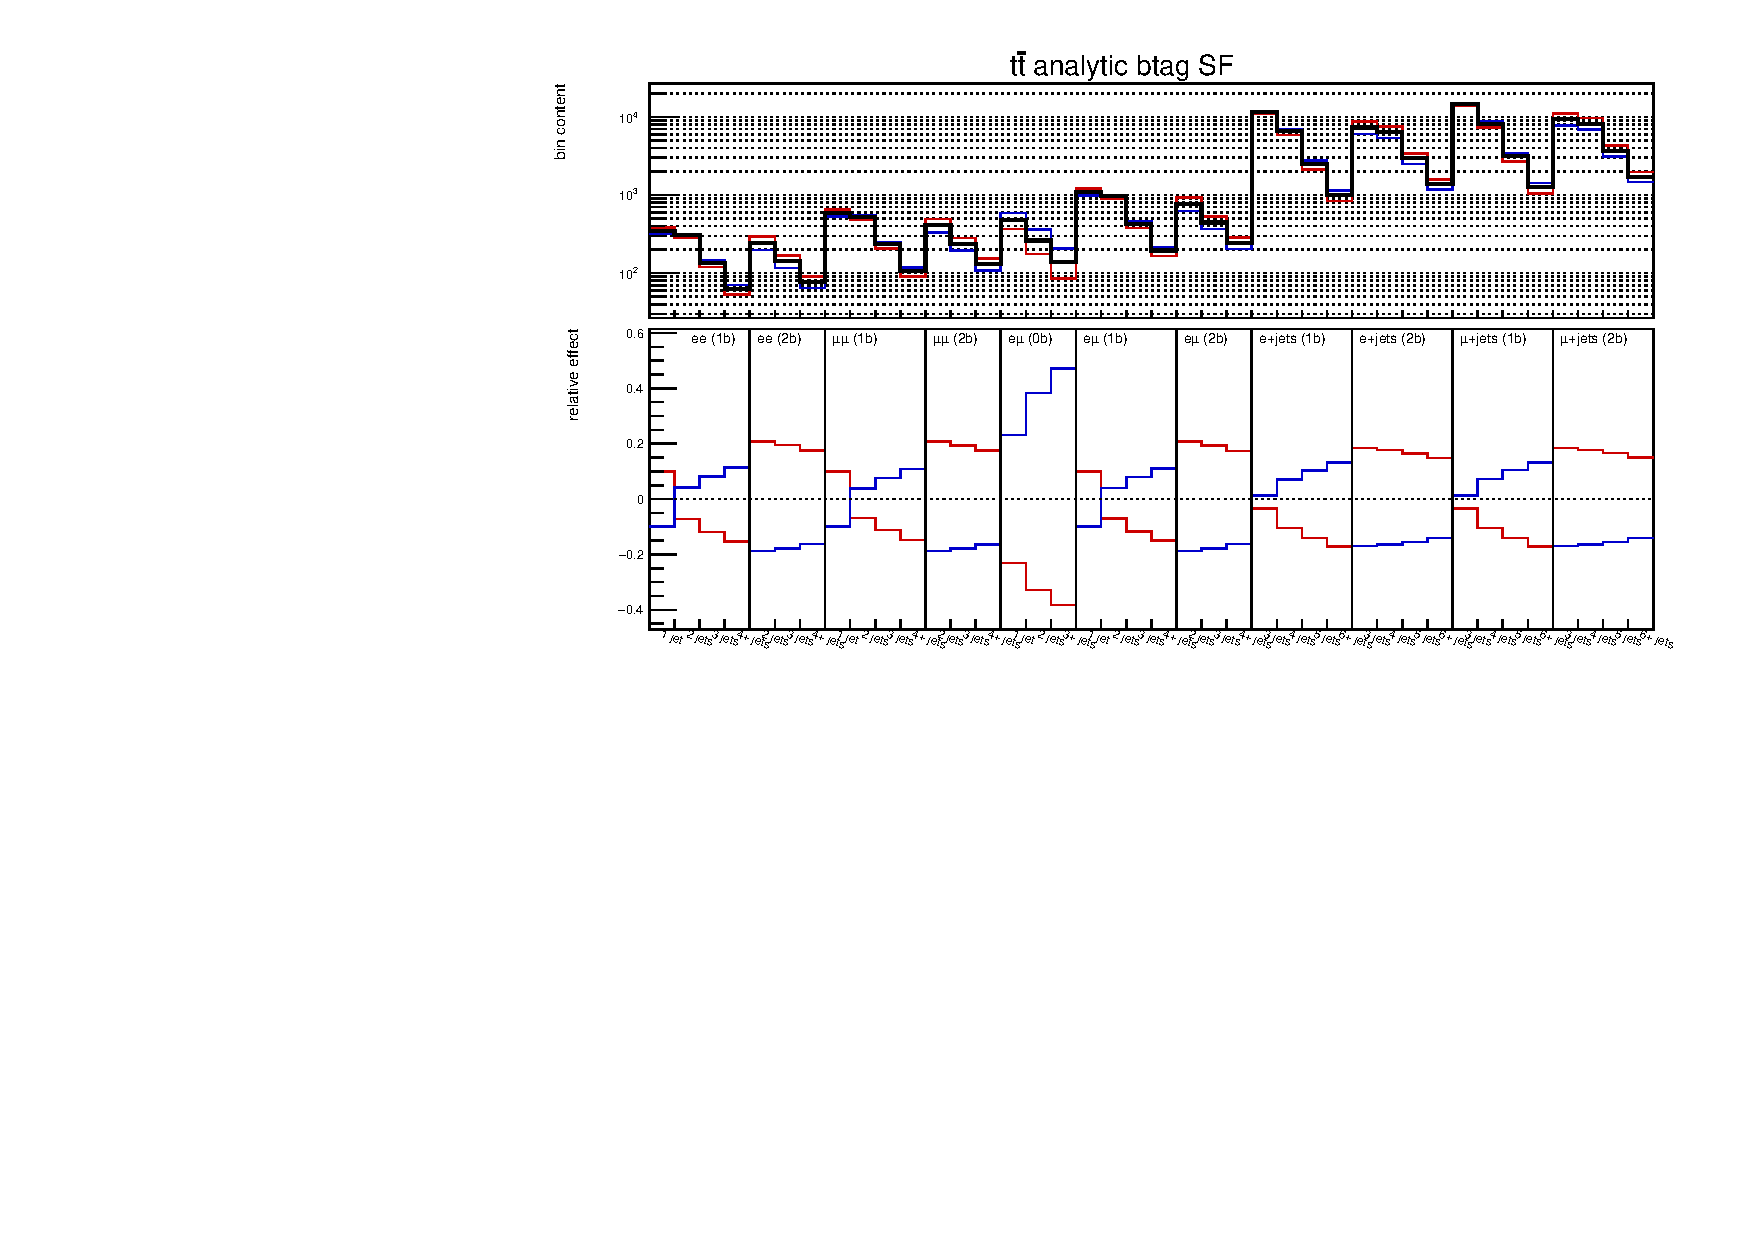
\includegraphics[width=0.8\textwidth]{figures/ttxs/scalefactors/btagsf_id_tt.pdf}
    \caption{
       \textbf{b tagging scale factor variation.} The effect of varying the b tagging scale factor $f_b$ in \ttbar MC by an arbitrary value of $\pm 0.1$, shown for the number of jets in the 11 fit categories. \todo{prettify figure}
    }
    \label{fig:ttxs:btagsf}
\end{figure}

Note that any dependence of $\epsilon_b$ on the jet kinematics factorizes out as long as said dependency is the same in data and MC. Possible kinematic dependencies of the ratio $f_b$ are neglected; since no kinematic information is used in the fit, this is deemed acceptable.

\paragraph{Lepton identification uncertainty}

% TODO: the structure is kinda shit here - scale factors + uncertainty + cross check. maybe try to merge some of these?

The uncertainty assumed on the lepton identification scale factors comes from two different sources: First, an inherent uncertainty originating in the tag-and-probe method (as described in \cref{sec:ttxs:scalefactors}) is considered. It consists of statistical uncertainties from both data and simulation, a systematic uncertainty derived from a comparison with a different Z+jets simulation sample produced at NLO in QCD, and another systematic uncertainty due to the choice of fitting function. Together, they make up for an uncertainty of $\sim 0.8\% \, (0.5\%)$ on the electron (muon) scale factors in the bulk of the phase space, and can rise up towards $\sim 5\%$ for high lepton \pt.

Secondly, it is taken into account that the scale factor between data and simulation might be slightly different in the Z+jets selection used for the T\&P method and the \ttbar selection used for the measurement of the cross section. The most important reason for this is the requirement of (b tagged) jets in almost all considered categories, as well as the requirement for at least three jets in the lepton+jets channels. 

This effect has been studied at CMS in the past and the difference found to be less then 0.5\% for muons and 1.0\% for electrons. Taking a conservative approach, these values are used as an additional component in the respective uncertainties.

\paragraph{Pileup uncertainty}

As described in \cref{sec:ttxs:scalefactors}, three different pileup-related variables are employed to reweight the simulation to the observed data, and the average of the three weights is used as the nominal value. This method is repeated using only one of the variables - the number of good reconstructed vertices $n_{\mathrm{PV}}$ - and the difference in expected yields treated as an uncertainty. It should be noted that this difference was found to be larger then the more common method of estimating pileup-related uncertainties, which consists of deriving a theoretical expectation for the number of interactions depending on the total inelastic proton-proton cross section, and varying this number by its experimental uncertainty.

\paragraph{Jet energy uncertainties}

Uncertainties in the jet energy calibration are split into 26 different sources concerning different experimental and theoretical effects, following the standard CMS procedure outlined in \citere{CMS:JME-13-004}. 17 of these sources are found to be non-negligible and included in the fit. These sources include, among others, uncertainties due to jet \pt resolution and jet flavour composition, statistical uncertainties in the derivations of the energy corrections, and residual differences between data and simulation.

\paragraph{Trigger uncertainties}

Since the trigger scale factors are derived using the tag-and-probe method in the same way as the lepton scale factors, similar uncertainties are applied, including the extrapolation uncertainties of 0.5\% for muons and 1.0\% for electrons. The only difference is that in the dilepton channels the uncertainties need to be propagated according to \cref{eq:ttxs:triggersf}. This has the effect of greatly reducing the impact of the trigger uncertainties in those channels compared to the lepton ID uncertainties, since the nominal per-event trigger efficiency is already very close to one.

\paragraph{Matrix element scale uncertainties}

The theoretical predictions of both signal and background are calculated using matrix elements at either LO or NLO in perturbative QCD, matched to a parton shower. Since this effectively means truncating the perturbative expansion of the scattering amplitude at a given power in the strong and electroweak coupling constants, the effect of higher-order terms is neglected in the calculation.

At the same time, the necessity of renormalization of divergent diagrams and factorization of non-perturbative contributions introduces non-physical parameters into the prediction in the form of the renormalization and factorization scales $\mu_R$ and $\mu_F$. These parameters are usually set to typical energy scales of the considered process, and might also depend on the event kinematics (dynamic scales).

To estimate possible errors due to these missing terms as well as due to the choice of scales, the scales $\mu_R$ and $\mu_F$ are varied separately by a factor of 2 up and down, and the resulting change in simulation is taken as an uncertainty in the form of shape templates \cite{Cacciari:2004}. In order to not double-count uncertainties in the cross section prediction for the backgrounds (see below), but keep possible rate variations due to acceptance effects, the templates are normalized to the nominal cross section values before any selection cuts are applied. Different physical processes are considered to be uncorrelated since they are produced with different generators and at different orders. 

\paragraph{PDF uncertainties}

The parton distribution functions (PDFs) used to evaluate the non-perturbative contribution of the proton-proton collision have systematic uncertainties attached. They are estimated by independently reweighting the simulation to 100 different replicas of the used NNPDF 3.1 PDF set and taking the envelope of the resulting changes, following the recommendations of the PDF4LHC working group \cite{Butterworth:2015oua}. Additionally, the effect of the choice of the strong coupling constant in the PDF is assessed using a similar reweighting, and attached as a separate nuisance parameter. Analogously to the matrix element uncertainties, the resulting variations are normalized before any selection cuts to keep acceptance and shape effects while not double-counting cross section changes.

\paragraph{Parton shower uncertainties}

Furthermore, the parton shower model used for the predictions is only accurate at leading-log (LL) as well as leading color (LC) in QCD (cf. \cref{sec:mc:showering}) and thus requires appropriate uncertainties. For this purpose, the scales at which the strong coupling constant is evaluated are varied up and down by a factor 2 separately for initial and final state radiation and for different processes, and the resulting changes propagated to the fit as shape templates.

\paragraph{ME/PS matching uncertainty}

For the simulation of the \ttbar signal, an additional uncertainty concerning the matching between matrix element simulation in \powheg and parton showering in Pythia is considered. This is done by varying the $h_{\mathrm{damp}}$ parameter in \powheg controlling the amount of radiation generated at matrix element level, following \citere{CMS:TOP-16-021}.

\paragraph{Background cross section uncertainties}

For the cross sections of the different processes, log-normal rate uncertainties are assigned based on the process and order at which it was calculated. Specifically, a 15 \% uncertainty is used for the single-t background since it is generated fully at NLO with a NNLO prediction for the cross section, while uncertainties of 20 \% and 30 \% are used for Z+jets as well as W+jets and Diboson, respectively, since these samples are only generated at LO. Additionally, for the fully data-driven QCD background, two separate nuisance parameters for the electron+jets and muon+jets channels are defined, covering a conservative uncertainty of 30 \% each.

\paragraph{Background statistical uncertainties}

Finally, since the background in this measurement is estimated either using MC simulation or data-driven methods, an independent statistical uncertainty needs to be attached to each bin, reflecting the finite number of events it contains. This is done using the method given in Ref.~\cite{Barlow:1993dm}. For MC backgrounds, these uncertainties are minuscule; however, they are non-negligible for the data-driven QCD background due to the limited data statistics used there.


\section{Fit results}
\label{sec:ttxs:fitresults}

\begin{figure}[!ht]
\centering
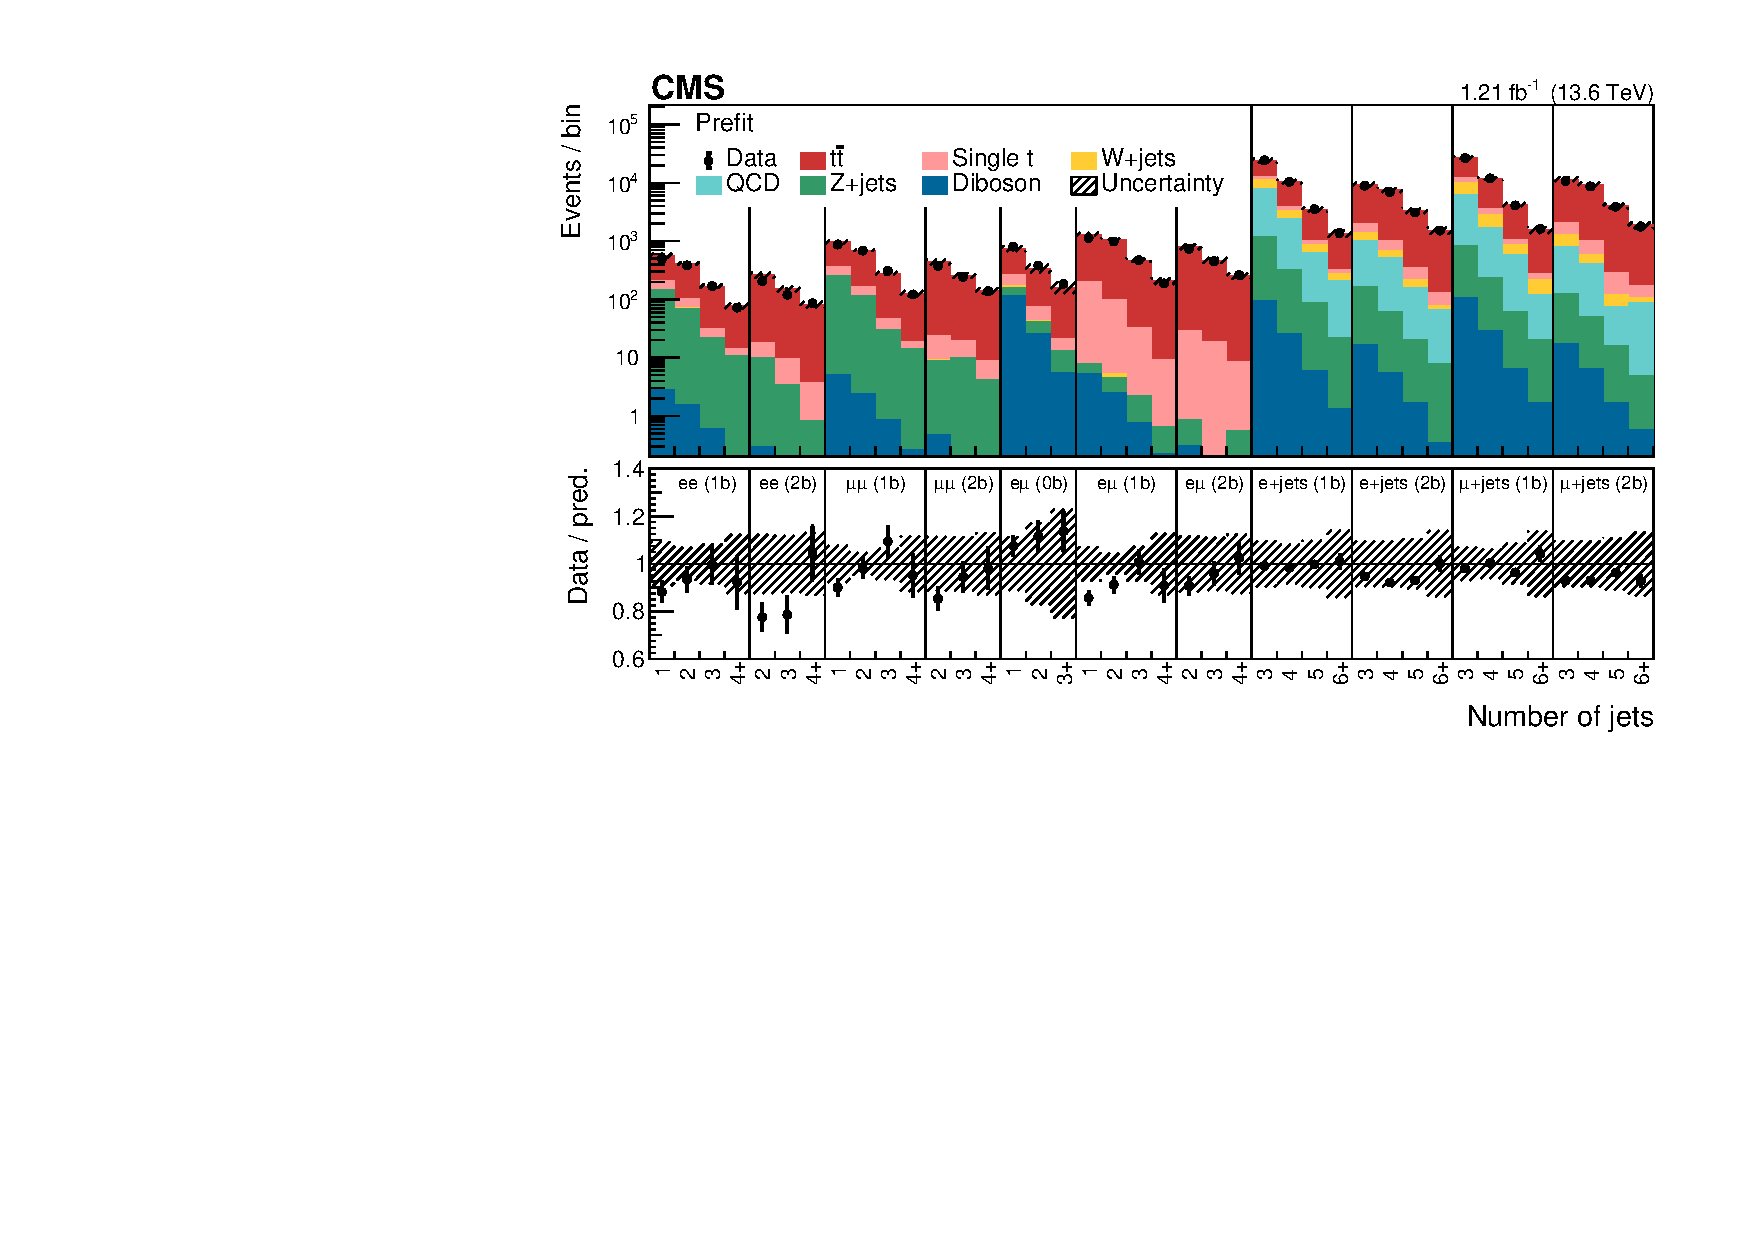
\includegraphics[width=0.99\textwidth]{figures/ttxs/prefithist.pdf}
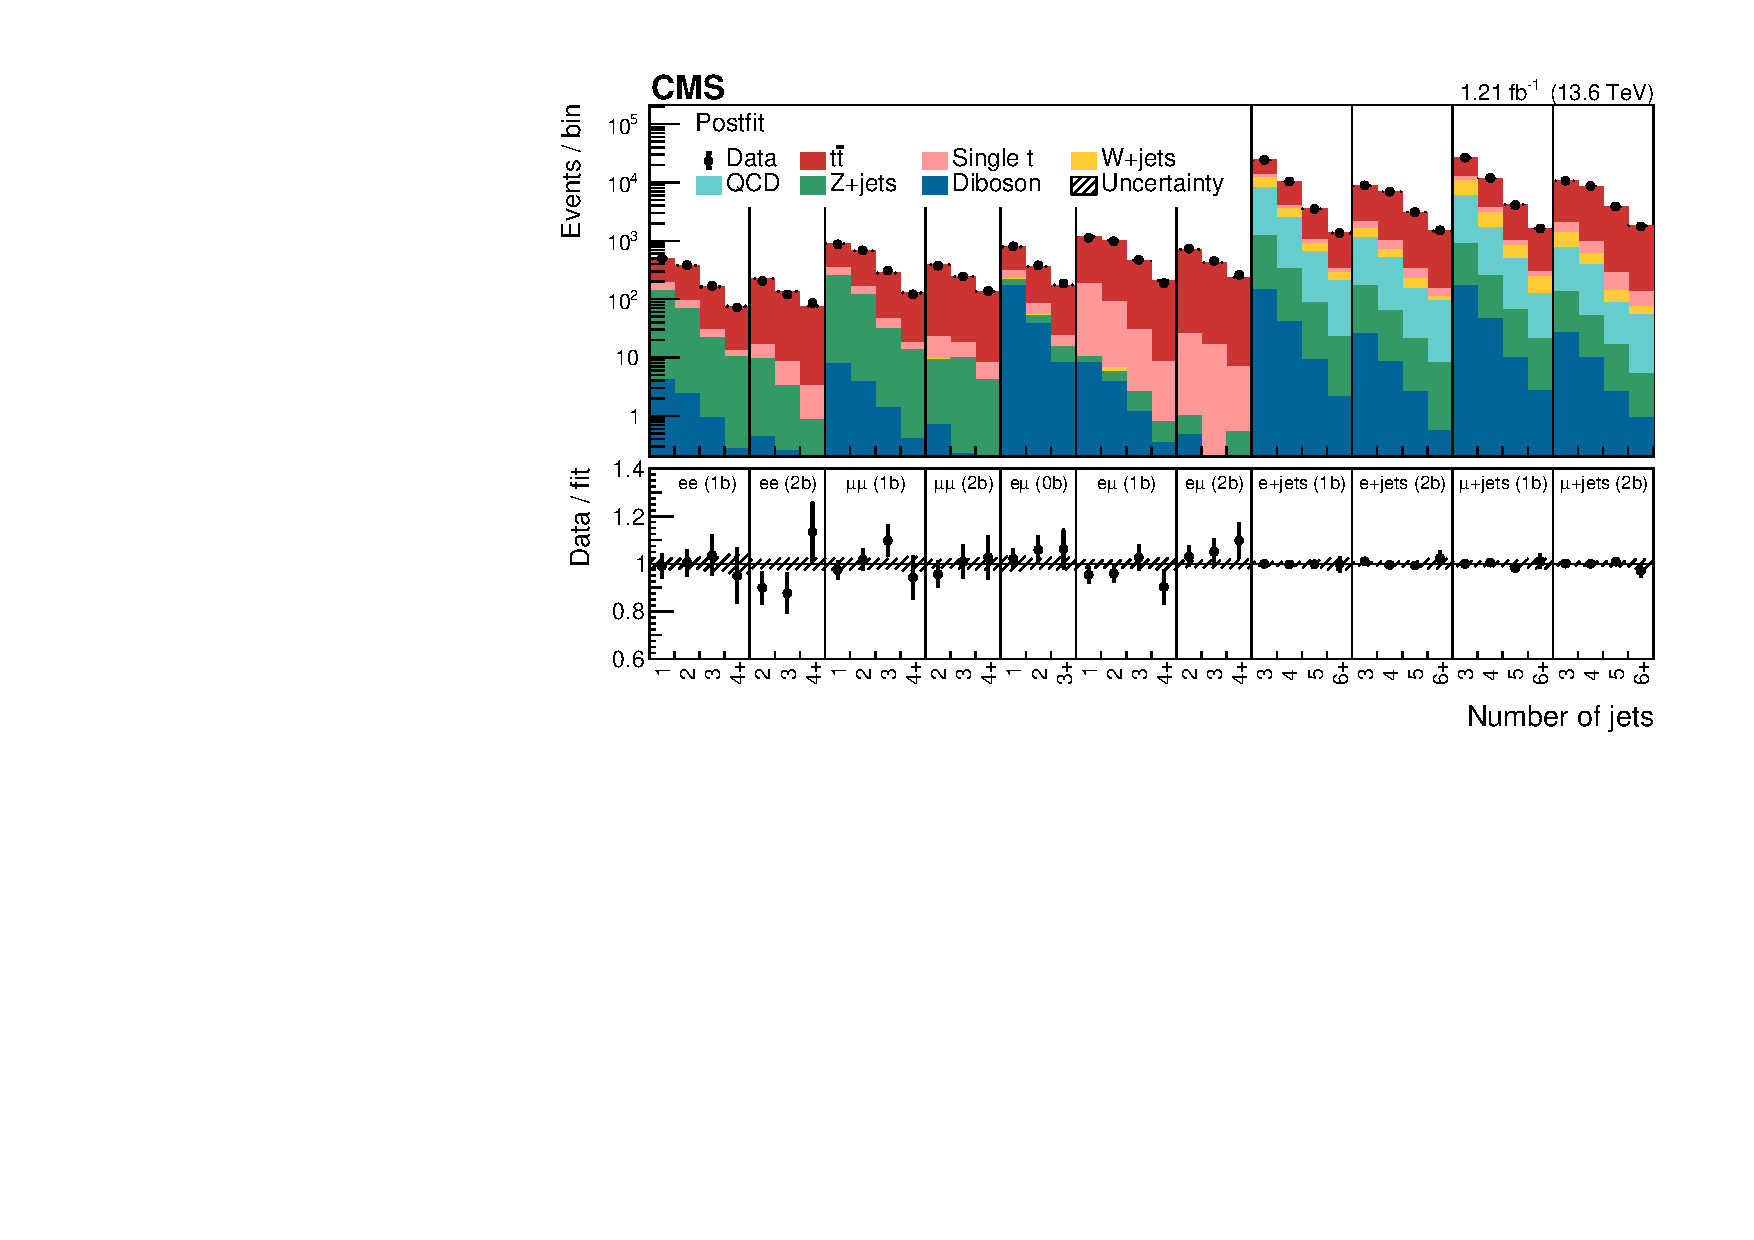
\includegraphics[width=0.99\textwidth]{figures/ttxs/postfithist.pdf}

\caption{
   \textbf{Comparison of data and simulation before and after the fit.} The distribution of the number of jets in the different fit categories is shown for data and simulation before (top) and after the likelihood fit (bottom). The fit greatly improves the agreement and strongly constrains the background uncertainties.
}
\label{fig:ttxs:prepostfit}
\end{figure}

Performing the fit yields a \ttbar signal strength of $r = 0.958 \pm 0.025$, where the uncertainty includes statistical and all systematic contributions, except for the 2.1\% uncertainty on the luminosity. This corresponds to an inclusive \ttbar cross section of

\[
    \sigmatt = 882 \pm 23 \, \text{(stat.+syst.)} \pm 20 \, \text{(lumi.)} \, \text{pb}
\]

The result is in agreement within one standard deviation with the standard model prediction of $\sigmatt^{\text{pred}} = 921^{+29}_{-37} \, \text{pb}$.

Fig.~\ref{fig:ttxs:prepostfit} shows the agreement between data and simulation before and after the fit. It can be immediately seen that the fit greatly reduces the uncertainty on the prediction by constraining systematic uncertainties and simultaneously improves the agreement compared to the data. 

Of particular note here is the free-floating b tagging efficiency (compare sec.~\ref{sec:ttxs:systematics}), whose effect can be directly read off from the categorization in the number of b jets: Before the fit (Fig.~\ref{fig:ttxs:prepostfit} top), the event yield for two or more b jets is overestimated in the simulation, while the yield for zero b jets is underestimated. This suggests that the b tagging efficiency is slightly lower in the data than assumed in the simulation. Indeed, the fit confirms this: the b tagging scale factor between data and simulation in the phase space of this measurement is measured to be $f_b  = 0.980 \pm 0.009$. As a result, after the fit (Fig.~\ref{fig:ttxs:prepostfit} bottom), the event yields agree in all b jet categories.

\subsection{Statistical checks}

To better understand the sources of systematic uncertainty, as well as the contributions of the different measurement channels, the fit is repeated twice, restricted to either the dilepton or the \ljets channels. For both cases as well as the combination, the contribution of different groups of nuisance parameters is calculated as explained in \cref{sec:methods:stat} \todo{actually add this info there}. The results can be found in \cref{tab:ttxs:systematics}, where it can be seen how the combination of channels helps to reduce the total uncertainty. 

\begin{table}[!ht]
\centering\renewcommand\arraystretch{1.1}
\begin{tabular}{l@{}c c c}
    Source & Full measurement & dilepton only & \ljets only\\
    \hline
    Lepton ID efficiencies & 1.6 & 2.4 & 1.0 \\
    Trigger efficiency & 0.4 & 0.0 & 0.5 \\
    JES & 0.7 & 0.7 & 1.0 \\
    b tagging efficiency & 1.0 & 0.4 & 1.8 \\
    Pileup reweighting & 0.5 & 0.0 & 1.0 \\
    ME scale, \ttbar & 0.5 & 0.4 & 0.6 \\
    ME scale, backgrounds & 0.1 & 0.1 & 0.3 \\
    ME/PS matching & 0.2 & 0.2 & 0.4 \\
    PS scales & 0.4 & 0.9 & 0.6 \\
    PDF and \alphas & 0.3 & 0.4 & 0.4 \\
    Single t background & 1.1 & 1.2 & 0.8 \\
    Z+jets background & 0.3 & 0.1 & 0.0 \\
    W+jets background & 0.0 & 0.0 & 0.1 \\
    Diboson background & 0.4 & 0.4 & 0.0 \\
    QCD multijet background & 0.3 & 0.0 & 0.5 \\
    Statistical uncertainty & 0.5 & 1.2 & 0.5 \\ \hline
    Combined uncertainty & 2.6 & 3.3 & 3.0 \\ \hline
    Integrated luminosity & 2.3 & 2.3 & 2.3 \\
\end{tabular}
\caption{
    \textbf{Sources of systematic uncertainty.} The relative per-cent contribution of different groups of sources of systematic uncertainty for the full measurement as well as for restrictions to the dilepton and \ljets channels only. They are calculated according to \cref{sec:methods:stat} and do not take correlations between the different groups into account.
}
\label{tab:ttxs:systematics}
\end{table}

Furthermore, the nuisance parameter pulls, constraints and impacts, as defined in \cref{sec:methods:stat}, are shown in \cref{fig:ttxs:impacts}. One can see here especially how the electron identification scale factors, which are the leading impact, are constrained by the combination of channels, while the same is not true of the muon identifaction scale factors due to their lower pre-fit uncertainty.

\begin{figure}[!ht]
    \centering
    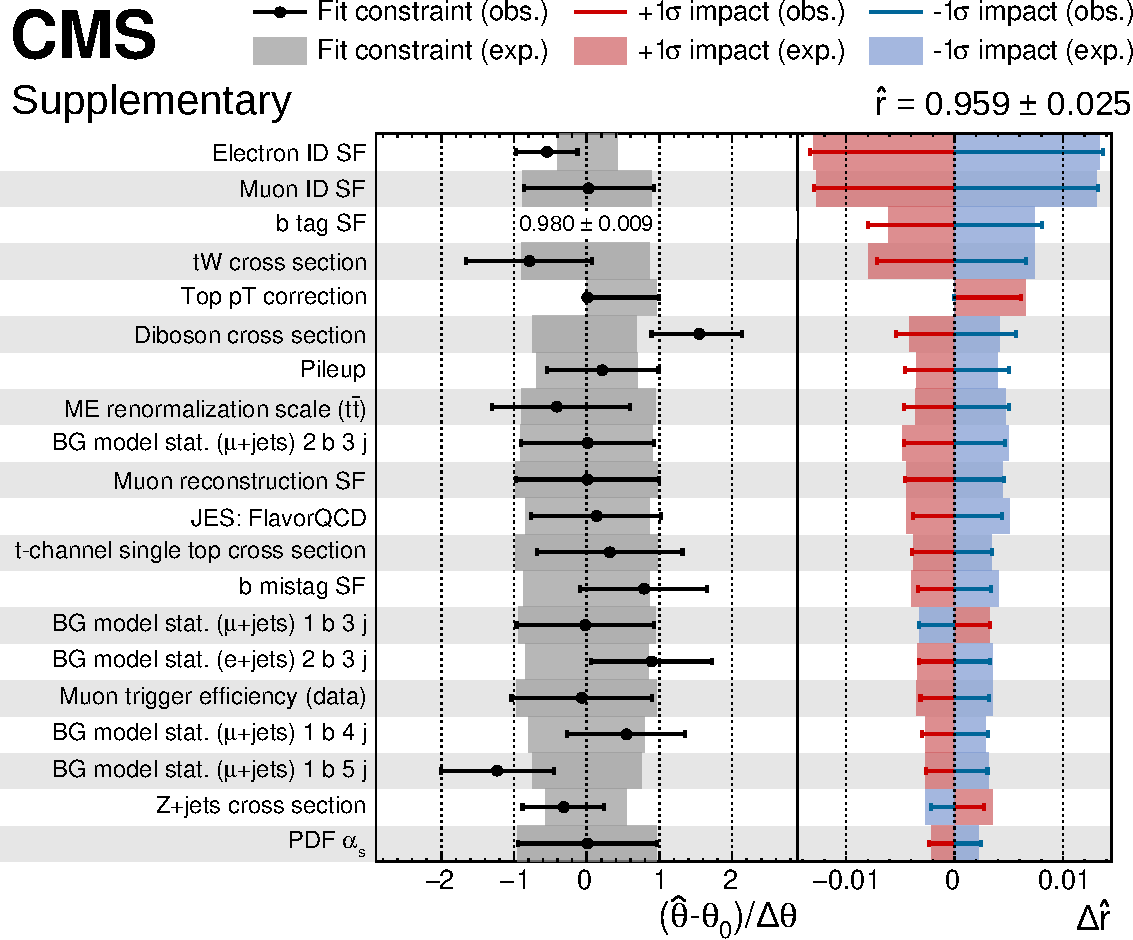
\includegraphics[width=0.9\linewidth]{figures/ttxs/impacts_v2.pdf}
    \caption{\textbf{Nuisance parameter pulls, constraints and impacts.} The expected and observed values are shown as shaded bands and error bars, respectively. Nuisance parameters are sorted by their observed impact on the signal strength $r$. For the b tagging scale factor, for which no pre-fit uncertainty is defined, the post-fit uncertainty is shown instead of the pull.}
    \label{fig:ttxs:impacts}
\end{figure}


%\subsection{Lepton efficiency check}

\subsection{Top quark mass dependence}
\label{sec:ttxs:topmass}

An additional source of uncertainty that has not been considered so far is the choice of top quark mass in the \ttbar MC simulation. It affects the selection efficiency indirectly via the \pt cuts on leptons and jets, with higher top quark mass values leading to harder spectra and thus to larger efficiencies.

Contrary to other uncertainty sources, the top quark mass is not profiled in the likelihood fit. Instead, the dependence of the extracted \ttbar cross section is explicitly quantified as a function of the top quark mass by shifting its value in simulation by $\pm \SI{3}{\GeV}$ from its defaulf of $\mt = \SI{172.5}{\GeV}$.
The extraction of \sigmatt is then repeated and the dependence on \mt extracted through a simple linear fit.

For an upwards shift of $\Delta \mt = \SI{1}{\GeV}$, the \ttbar cross section is found to shift downwards by \SI{8.5}{\pb}, and vice versa. If one takes the current experimental uncertainty of \SI{0.3}{\GeV}~\cite{PDG:2022pth} as an allowed range for \mt, this would lead to an additional uncertainty on \sigmatt of 0.3\%.
% todo: impacts and GOF
% lepton SF consistency check
% tt curve

\section{Summary and Outlook}

\begin{figure}[!ht]
    \centering
    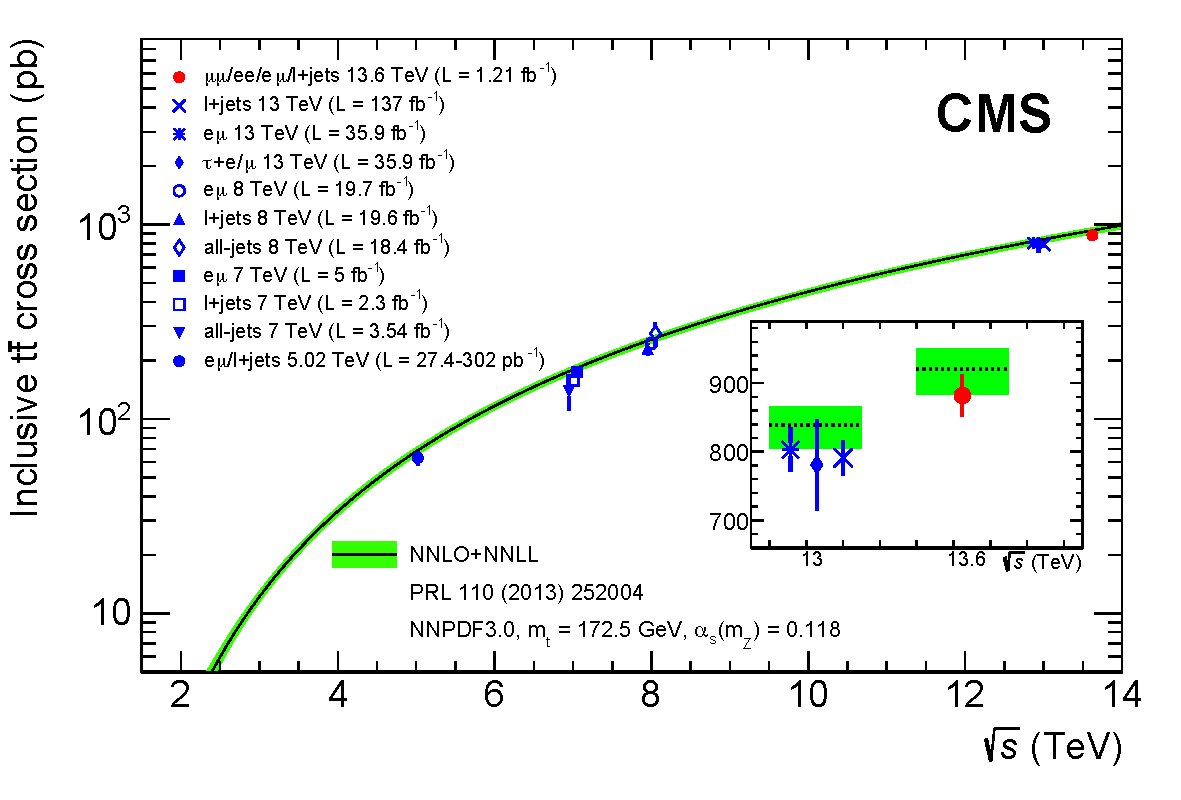
\includegraphics[width=0.8\linewidth]{figures/ttxs/tt_curve.pdf}
    \caption{\textbf{Summary of \sigmatt measurements.} An overview of inclusive \ttbar cross section measurements at CMS at different center-of-mass energies~\cite{CMS:TOP-11-007, CMS:TOP-14-018, CMS:TOP-12-006, CMS:TOP-13-004, CMS:TOP-17-001, CMS:TOP-18-005, CMS:TOP-20-001, CMS:TOP-20-004} as well as comparison to the SM prediction~\cite{Czakon:2013goa}. This measurement is displayed as the red dot.}
    \label{fig:ttxs:ttcurve}
\end{figure}

In this chapter, the inclusive \ttbar cross section is measured for the first time at a center-of-mass energy of \sqrtsRIII. Data corresponding to an integrated luminosity of \lumiRIII from the beginning of LHC Run~3 are analyzed. Despite this comparatively small amount of data, a total precision of ca. 3\% with respect to the inclusive cross section is achieved.

\cref{fig:ttxs:ttcurve} compares the result of this chapter to other inclusive \ttbar cross section measurements performed by CMS at other center-of-mass energies~\cite{CMS:TOP-11-007, CMS:TOP-14-018, CMS:TOP-12-006, CMS:TOP-13-004, CMS:TOP-17-001, CMS:TOP-18-005, CMS:TOP-20-001, CMS:TOP-20-004}, as well as to the SM prediction~\cite{Czakon:2013goa}. The precision is comparable to other measurements at $\sqrt{s} = 7$, $8$, and $\SI{13}{\TeV}$, some of them with significantly higher integrated luminosities. All results are in agreement with the SM.

This measurement was designed specifically for the earliest data of Run~3, and this is what allows it to reach comparatively high precision even though not all calibrations were available. In particular, b tagging and lepton efficiencies can be constrained in situ using the combination of dilepton and \ljets channels as well as the categorization by number of b-tagged jets. No large inconsistencies for any of the considered physics objects were found. The measurement was made public in September of 2022 just two months after the start of Run~3 and constituted the first public result of LHC Run~3. At the time, it provided a valuable first proof that the data taken in Run~3 was of high quality and ready for physics.

The next step for this result would be to transfer the technique developed in this work to well-understood data and high integrated luminosities in order to achieve the highest precision possible for \sigmatt. Such a measurement will certainly be dominated by systematic uncertainties, most importantly the luminosity and the lepton identification efficiencies (as already partly the case here). The channel combination method developed here could help reduce the latter of these through an in situ constraint, while the former is orthogonal to the analysis strategy and its reduction requires more precise luminosity measurements. It will likely also be necessary to study the different sources of uncertainty in more detail, and investigate whether some of them can be reduced through more careful calibrations.

Additionally, one could try to use such a high-precision \ttbar cross section measurement to indirectly measure the top quark mass, one of the fundamental parameters of the Standard Model, by comparing the measured value to SM predictions for different top quark masses. For this purpose, it would be important to reduce the dependence on the top quark mass in simulation (c.f. \cref{sec:ttxs:topmass}), for example by reducing the \pt requirements on leptons and jets as much as experimentally feasible. All of this is, however, not part of this thesis and material for future work.
% what about outlook to higher lumi values? easy to do...